\documentclass[12pt]{article}
\usepackage{graphicx} % Required for inserting images
\usepackage{amsmath, amssymb}
\usepackage{tikz}
\usetikzlibrary{arrows.meta, positioning}
\usepackage{subfig}
\usepackage[round]{natbib}
\usepackage[margin = 2.5cm]{geometry}
\usepackage{url}
\usepackage{xr}
\externaldocument{appendix}

%\title{Deriving Complete Constraints in Hidden Variable Models}
%\author{Michael C.~Sachs \and Erin E.~Gabriel  \and Robin J.~Evans \and Arvid Sjölander}
%\date{\today}

\newcommand\indep{\protect\mathpalette{\protect\independenT}{\perp}}
\def\independenT#1#2{\mathrel{\rlap{$#1#2$}\mkern2mu{#1#2}}}

\newtheorem{proposition}{Proposition}
\newtheorem{definition}{Definition}
\newtheorem{example}{Example}
\newtheorem{condition}{Condition}
\newtheorem{remark}{Remark}

\def\Pr{{\mathrm{P}}}
\def\Pdo{{\mathrm{P}^*}}

\DeclareMathOperator{\Anobs}{Anobs}
\DeclareMathOperator{\Paobs}{Paobs}
\DeclareMathOperator{\Chobs}{Chobs}
\DeclareMathOperator{\Disobs}{Disobs}



\tikzset{rv/.style={circle, draw, inner sep=0.5mm, minimum size=7mm}}
\tikzset{fv/.style={draw}}

\newcommand{\bW}{\boldsymbol{W}}
\newcommand{\bU}{\boldsymbol{U}}
\newcommand{\bV}{\boldsymbol{V}}
\newcommand{\bR}{\boldsymbol{R}}
\newcommand{\bS}{\boldsymbol{S}}
\DeclareMathOperator{\rank}{rank}
\DeclareMathOperator{\Do}{do}
\DeclareMathOperator{\Pa}{Pa}
% \DeclareMathOperator{\Do}{\mbox{do}}
% \DeclareMathOperator{\Pa}{\mbox{Pa}}

\setcounter{MaxMatrixCols}{20}

\def\spacingset#1{\renewcommand{\baselinestretch}%
{#1}\small\normalsize} \spacingset{1}
\newcommand{\blind}{0}

%\usepackage{setspace}
%\doublespacing

\begin{document}


\if1\blind
{
  \title{\bf Deriving Complete Constraints in Hidden Variable Models}
  \author{Michael C. Sachs$^1$\thanks{EEG and MCS are funded in part by NNF Grant NNF22OC0076595 and the Pioneer Centre for SMARTbiomed}, Erin E. Gabriel$^1$, \\
  Robin J. Evans$^2$,
  Arvid Sj\"olander$^3$\\  
\footnotesize 1:Section of Biostatistics and the Pioneer Centre for SMARTbiomed, \\ \footnotesize University of Copenhagen, Copenhagen, Denmark \\
\footnotesize 2:Department of Statistics, University of Oxford, Oxford, United Kingdom \\
\footnotesize 3:Department of Medical Epidemiology and Biostatistics, Karolinska Institutet, Stockholm, Sweden \\
\footnotesize corresponding author: michael.sachs@sund.ku.dk}
  \maketitle
} \fi 

\if0\blind
{
  \bigskip
  \bigskip
  \bigskip
  \begin{center}
    {\LARGE\bf Deriving Complete Constraints in Hidden Variable Models}
\end{center}
  \medskip
} \fi

\bigskip


\begin{abstract}
Hidden variable graphical models can sometimes imply constraints on the observable distribution that are more complex than simple conditional independence relations. These observable constraints can falsify assumptions of the model and can be used to constrain estimation procedures to improve statistical efficiency. Knowing the complete set of observable constraints is thus ideal, but this can be difficult to determine in many settings.  In models with categorical observed variables and a joint distribution that is completely characterized by linear relations to the unobservable response function variables, we develop a systematic method for deriving the complete set of observable constraints. We illustrate the method in several new settings, including ones that imply both inequality and equality constraints. \\
\noindent \textit{Keywords:} Causal models, Hidden variables, Constraints, Directed acyclic graphs.
\end{abstract}

\newpage
\spacingset{2}
\vspace{-1cm}

\section{Introduction}


The assumption of a structural model with hidden variables can rule out particular joint distributions not only due to observable conditional independence relations but also due to more complex observable conditions, which may not be clear from inspection of the causal model alone. These observable constraints can be used to falsify a structural model in settings where the data contradict these constraints. The instrumental inequalities first discussed in \citet{pearl1995testability} for the all binary instrumental variable (IV) setting are the most well-known example of these more complex constraints in the form of inequalities, while the ``Verma" constraints \citep{verma2022equivalence} are a well-known example of observable and thus falsifiable equality constraints representing a more general notion of conditional independence. 

In the general IV setting, \citet{bonet2001instrumentality} derived inequality constraints showing that, in cases with an IV with more than two categories, there are more observable constraints beyond the binary IV constraint set. Within the specific setting of all discrete observed variables within the classical trivariate IV setting he developed a method for deriving constraints on the observed data distribution implied by the causal assumptions and proved that these are the ``sufficient" set of constraints. We will use the term ``complete'' to refer to what \citeauthor{bonet2001instrumentality} called sufficient, but the meaning remains the same, i.e.~all observable and therefore falsifiable constraints implied by a structural model.  

The \citet{bonet2001instrumentality} method is what \citet{evans2012graphical} called the ``computationally intensive linear programming technique''. As pointed out by \citet{evans2012graphical}, complete constraints are difficult to derive without using such techniques or algebraic variable elimination algorithms, e.g., Fourier-Motzkin elimination, which become infeasible for moderately sized state spaces. Although other attempts have been made, such as \citet{kang2006inequality}, the derived constraints are not complete. This is also true for the \emph{nested Markov} characterization which, by construction, only involves equality constraints \citep{evans2019smooth, shpitser2012parameter, verma2022equivalence, richardson2023nested}.

We conceptually extend the method of \citet{bonet2001instrumentality} beyond the IV setting, which due to increased computational power is now feasible in many more settings. We prove that within the class of models that we refer to as ``linear", as defined in \citet{duarte2023automated}, our method provides the complete set of observable constraints. Linear here refers to settings with categorical observed variables and a joint distribution that is completely characterized by linear relations to the unobservable response function variables \citep{balke1994counterfactual, sachs2023general}; in our setting, these are the graphs of c-degree one (Definition \ref{def:cdeg}). We also relate the equality constraints that we derive to the nested Markov model, and we show that the method can be used outside the ``linear" class to derive at least some of the constraints. We illustrate our method in several examples, providing, to our knowledge, novel constraints. All proofs are in the Appendix, Section \ref{appendix:proofs}, and software implementing the method is publicly available on GitHub at \url{https://github.com/sachsmc/meraconstraints}.



\section{Notation and Preliminaries}
\subsection{Notation}
Let $\mathcal{G}(\bV, \bU)$ be a hidden variables directed acyclic graph (DAG) representing a nonparametric structural equations model (NPSEM) \citep{Pearl2000causality}, over variables $\bW = \bV \cup \bU$ where $\bU$ are unobserved and $\bV$ are observed. We assume that all variables in $\bV$ are discrete and finite, but no assumptions are made about $\bU$. We will write $\bV_i$ (or some other index) to denote a subset of $\bV$, and $V_i$ a single element of $\bV$. Let $|\bV|$ denote the cardinality of the set $\bV$, and when used for a single variable, for example $|V_i|$, let it denote the number of possible values that variable $V_i$ can take, i.e., the cardinality of its domain. Let $\Paobs(\bV_i)$ denote the union of the sets of observed parents of each variable in the set $\bV_i$ and $\Pa(\bV_i)$ denote the union of the sets of all, observed or unobserved, parents of each variable in the set $\bV_i$. Let $\Anobs(\bV_i)$ denote the union of the sets of observed ancestors of each variable in $\bV_i$, where, as in \citet{evans2019smooth}, $V_2$ is an ancestor of $V_1$ if there is a sequence of directed edges $V_2 \rightarrow \cdots \rightarrow V_1$, and by definition, we include $V_1$ itself in the set of ancestors. Let $\Chobs(\bW_i)$ be the union of the sets of observed children of variables in $\bW_i$, where $W_1$ is a child of $W_2$ if and only if $W_2$ is a parent of $W_1$. Throughout, we assume that the observed distribution is strictly positive, i.e., $\Pr(\bV = v) > 0$ for all $v$, so that all conditional probabilities below are well defined. The boundary case is discussed in Remark \ref{rmk:positivity}.


\subsection{Settings}
Our goal is to characterize the distribution $\Pr(\bV)$, known as the marginal model (because it is marginal with respect to $\bU$), in terms of constraints implied by the NPSEM for $(\bV,\bU)$. Following \citet{evans2016graphs}, Section 3.2, we can restrict our attention to a smaller class of hidden variables DAGs that satisfy the following two conditions.
\begin{condition} \label{A1}
All unobserved variables are exogenous, i.e., $\Pa(U_i) = \emptyset$ for all $U_i \in \bU$.
\end{condition}

\begin{condition} \label{A2}
The child set of each unobserved variable corresponds to a distinct
set of observed vertices of at least size 2. That is, for each $U_i \in \bU$, $|\Chobs(U_i)| \geq 2$, $\Chobs(U_i) \subseteq \bV$, and there is no other $U_j \in \bU$ such that $\Chobs(U_i) \subseteq \Chobs(U_j)$.
\end{condition}

By Lemmas 1--3 of \citet{evans2016graphs}\footnote{Here we use the references to the published version of these Lemmas, rather than the arXiv version. The arXiv versions are Lemmas 3.7--3.9.}, DAGs where these conditions do not hold can be transformed to DAGs where they do hold without changing the implied marginal model. Briefly, the exogenization process replaces sequences of the form $W_1 \rightarrow U_1 \rightarrow V_1$ by $W_1 \rightarrow V_1$ without changing the marginal model, where $W_1$ could be observed or unobserved. Following exogenization, any unobserved variable $U_1$ whose child set is a subset of that of another unobserved variable $U_2$ can be absorbed into a common unobserved variable with child set equal to the union of child sets of $U_1$ and $U_2$. Examples of these transformations are given in Figures 4 and 5 of \citet{evans2016graphs}.



\begin{definition} \label{def:districts}
Let $\mathcal{G}(\bV, \bU)$ be a hidden variables DAG that by construction obeys Conditions \ref{A1} and \ref{A2}. Remove all edges that do not originate from variables in $\bU$. The sets of variables in $\bW$ that remain connected form a partition of $\bW$ called \emph{districts}. Denote $\mathcal{D}(\mathcal{G}) = \{D_1, \ldots, D_k\}$ the set of districts of $\mathcal{G}$. 
\end{definition}

This same concept is called a \emph{c-component} (short for confounded component) by \citet{tian2002testable}, while the term district is used in, e.g., \citet{richardson2003admgs}, \citet{evans2018margins}, and \citet {duarte2023automated}, which we will follow. We further define the c-degree of a district as follows.


\begin{definition}\label{def:cdeg}
Let $\mathcal{G}(\bV, \bU)$ be a hidden variables DAG that follows Conditions \ref{A1} and \ref{A2}. Let $D_j$ be a district in $\mathcal{G}(\bV, \bU)$. The \emph{c-degree} of $D_j$ is the number of hidden variables $U_i$ in $\bU$ that are in $D_j$. The c-degree of a DAG $\mathcal{G}(\bV, \bU)$ is the maximum of the c-degrees of its districts. 
\end{definition}

The example in Figure \ref{fig:district} illustrates the two definitions in this Section. The graph has three districts, one with c-degree 0 ($\{G\}$), one with c-degree 1 ($\{A, C, E, U_2\}$) and one with c-degree 2 ($\{B, D, F, U_1, U_3\}$). Thus, Figure \ref{fig:district} has c-degree 2. 



\begin{figure}[ht]
\begin{center}
  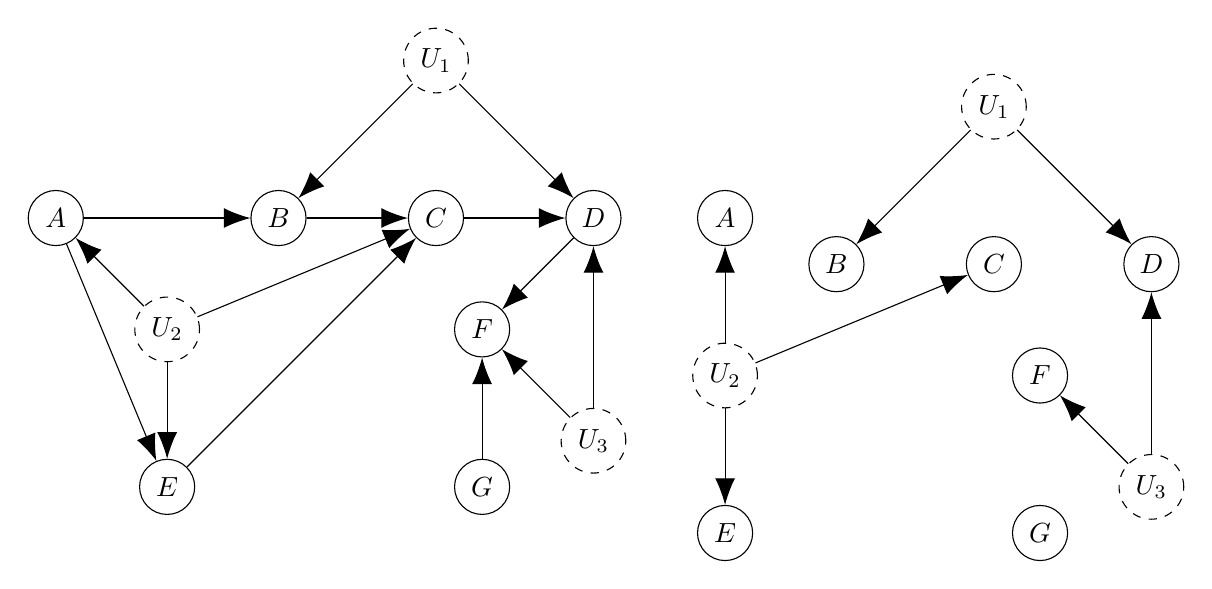
\begin{tikzpicture}[>=Stealth, node distance=2cm, on grid, auto]
\begin{scope}
  % Nodes
  \node (A) [rv] {$A$};
  \node[draw, circle, dashed] (U2) [below right= of A] {$U_2$};
  \node (B) [above right=of U2, rv] {$B$};
  \node (C) [right=of B, rv] {$C$};
  \node (D) [right=of C, rv] {$D$};
  
  \node (F) [below left=of D, rv] {$F$};
  \node (G) [below= of F, rv] {$G$};

  % unobserved variables (U1, U2, U3)
  \node[draw, circle, dashed] (U1) [above =of C] {$U_1$};
  
  \node[draw, circle, dashed] (U3) [below right=of F] {$U_3$};
\node (E) [below=of U2, rv] {$E$};
  % Arrows
  \draw [-{Latex[scale=2.0]}]  (A) -- (B);
  \draw [-{Latex[scale=2.0]}]  (E) -- (C);
  \draw [-{Latex[scale=2.0]}]  (C) -- (D);
  \draw [-{Latex[scale=2.0]}]  (D) -- (F);
  \draw [-{Latex[scale=2.0]}]  (A) -- (E);
  \draw [-{Latex[scale=2.0]}]  (B) -- (C);
  \draw [-{Latex[scale=2.0]}]  (G) -- (F);

  % Dashed arrows (unobserved variables)
  \draw [-{Latex[scale=2.0]}] (U1) -- (B);
  \draw [-{Latex[scale=2.0]}] (U1) -- (D);
  \draw [-{Latex[scale=2.0]}] (U2) -- (A);
  \draw [-{Latex[scale=2.0]}] (U2) -- (E);
  \draw [-{Latex[scale=2.0]}] (U2) -- (C);
  \draw [-{Latex[scale=2.0]}] (U3) -- (F);
  \draw [-{Latex[scale=2.0]}] (U3) -- (D);
    
\end{scope}
\begin{scope}[xshift = 8.5cm]
\node (A) [rv] {$A$};
  \node[draw,circle,dashed] (U2) [below= of A] {$U_2$};
  \node (B) [above right=of U2, rv] {$B$};
  \node (C) [right=of B, rv] {$C$};
  \node (D) [right=of C, rv] {$D$};
  
  \node (F) [below left=of D, rv] {$F$};
  \node (G) [below= of F, rv] {$G$};

  % unobserved variables (U1, U2, U3)
  \node[draw,circle,dashed] (U1) [above =of C] {$U_1$};
  
  \node[draw,circle,dashed] (U3) [below right=of F] {$U_3$};
\node (E) [below=of U2, rv] {$E$};
  % Dashed arrows (unobserved variables)
  \draw [-{Latex[scale=2.0]}] (U1) -- (B);
  \draw [-{Latex[scale=2.0]}] (U1) -- (D);
  \draw [-{Latex[scale=2.0]}] (U2) -- (A);
  \draw [-{Latex[scale=2.0]}] (U2) -- (E);
  \draw [-{Latex[scale=2.0]}] (U2) -- (C);
  \draw [-{Latex[scale=2.0]}] (U3) -- (F);
  \draw [-{Latex[scale=2.0]}] (U3) -- (D);
      
\end{scope}
\end{tikzpicture}
\end{center}
\caption{Example to illustrate Definitions \ref{def:districts} and \ref{def:cdeg}. The left figure is the original one, and the right figure has the edges originating from observed variables removed. The graph has three districts: $\{G\}$ with c-degree 0, $\{A, C, E, U_2\}$ with c-degree 1, and $\{B, D, F, U_1, U_3\}$ with c-degree 2. \label{fig:district}}
\end{figure}

\clearpage

\subsection{Transformations that may reduce the c-degree} \label{graphmod}

Different graphs can have the same marginal model. For example, the graph $X \rightarrow Y$ has the same marginal model as the graph in which $X$ and $Y$ share an unobserved parent. Such graphs are \emph{observationally} equivalent, although they need not be causally equivalent. Since our method gives complete constraints for graphs with c-degree one, it is useful to replace a graph by an observationally equivalent graph with a lower c-degree. We use two rules for this. The first, due to \citet[Theorem 26.4; see also Proposition 4 of \citealp{ansanelli2025observationalpartialordercausal}]{henson2014theory}, adds or removes an edge.

\begin{proposition}[HLP Proposition] \label{prop:hlp}
  Let $V_1$ and $V_2$ be observed vertices, and let $\mathcal{G}$ and $\mathcal{G}^+$ be DAGs that meet Conditions \ref{A1} and \ref{A2} and are identical except that $\mathcal{G}^+$ contains the edge $V_1 \to V_2$ and $\mathcal{G}$ does not.
  If:
  \begin{itemize}
      \item $\Pa(V_1) \subseteq \Pa(V_2)$;
      \item There exists a $U_1$ s.t. $\{V_1, V_2\} \subseteq \Chobs(U_1)$;
  \end{itemize}
  then $\mathcal{G}$ and $\mathcal{G}^+$ have the same constraints. Hence the edge $V_1 \to V_2$ may be added to $\mathcal{G}$ or removed from $\mathcal{G}^+$.
\end{proposition}

The two conditions hold in $\mathcal{G}$ if and only if they hold in $\mathcal{G}^+$, because only the parent set of $V_2$ differs between the two graphs. The second rule is the Strong Facet-Merging rule of \citet[Proposition 8; see also Proposition 15]{ansanelli2025observationalpartialordercausal}, translated into our notation. We state it in the direction that splits unobserved variables, which can reduce the c-degree.

\begin{proposition}[Strong Face Splitting] \label{prop:strong}
  Let $\mathcal{G}$ be a hidden variables DAG satisfying Condition \ref{A1}, with unobserved vertices $U_1, \ldots, U_k$. Let $C_1, \ldots, C_k$ and $D$ be sets of observed vertices such that $\Chobs(U_i) = C_i \cup D$ for $i = 1, \ldots, k$, and $D$ is nonempty and disjoint from every $C_i$; the sets $C_i$ need not be disjoint from each other. Suppose that:
  \begin{enumerate}
      \item $\Paobs(C_i) \cup C_i \subseteq \Paobs(d)$ for each $d \in D$ and $i = 1, \dots, k$;
      \item for every unobserved vertex $U_j$ with $j \notin \{1, \ldots, k\}$ such that $\Chobs(U_j)$ intersects $\bigcup_{i=1}^k C_i$ and is not contained in $\bigcup_{i=1}^k C_i$, we have $D \subseteq \Chobs(U_j)$.
  \end{enumerate}
  Define the \emph{split} graph $\mathcal{G}^*$ that has the same nodes and edges as $\mathcal{G}$, except that $U_1, \ldots, U_k$ and their edges are replaced by unobserved vertices $U^*_1, \ldots, U^*_{k+1}$ with $\Chobs(U^*_i) = C_i$ for $i = 1, \ldots, k$ and $\Chobs(U^*_{k+1}) = D$. Then $\mathcal{G}$ and $\mathcal{G}^*$ have the same constraints. Hence $U_1, \ldots, U_k$ in $\mathcal{G}$ may be split into $U^*_1, \ldots, U^*_{k+1}$ (face splitting).
\end{proposition}

To apply the proposition, choose $U_1, \ldots, U_k$ with at least one child in common, let $D$ be a nonempty subset of $\bigcap_i \Chobs(U_i)$, and let $C_i = \Chobs(U_i) \setminus D$. An unobserved vertex of $\mathcal{G}^*$ with a single child can be deleted, so after splitting, the transformations above restore Condition \ref{A2}. Together with Proposition \ref{prop:hlp}, Proposition \ref{prop:strong} includes the rule for splitting an unobserved vertex in Proposition 5 of \citet{evans2016graphs}.

Figure \ref{fig:ivequiv} shows an example. The left DAG has c-degree two. Since $\Pa(Z) = \{U_1\} \subseteq \Pa(X)$ and $U_1$ is a parent of both, Proposition \ref{prop:hlp} adds the edge $Z \rightarrow X$, which gives the center DAG. Proposition \ref{prop:strong} then splits $U_1$, with $k = 1$, $D = \{X\}$ and $C_1 = \{Z\}$. The first condition holds because $\Paobs(Z) \cup \{Z\} = \{Z\} \subseteq \Paobs(X)$, and the second because $U_2$ has no child in $C_1$. Both resulting unobserved vertices have a single child and are deleted, which leaves the instrumental variable DAG on the right. It has c-degree one, so our method gives the complete constraints of all three DAGs.

\begin{figure}[ht]
\centering
    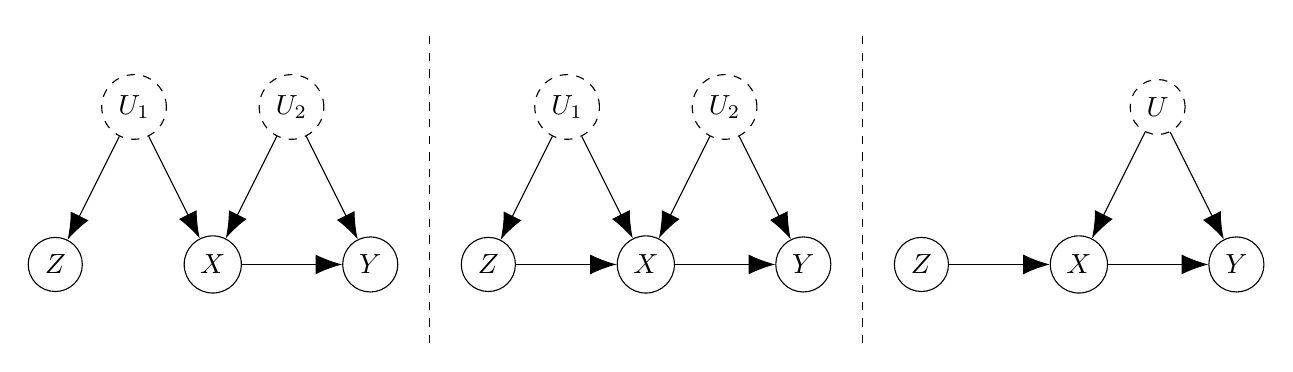
\begin{tikzpicture}
    \begin{scope}[xshift=-2cm]
    \node[draw, circle] at (2, 0) (X) {\(X\)};
    \node[draw, circle] at (4, 0) (Y) {\(Y\)};
    \node[draw, circle] at (0, 0) (Z) {$Z$};
    \node[draw, circle, dashed] at (1,2) (U1) {\(U_1\)};
    \node[draw, circle, dashed] at (3,2) (U2) {\(U_2\)};
    \draw [-{Latex[scale=2.0]}] (X) to (Y);
    \draw [-{Latex[scale=2.0]}] (U2) to (X);
    \draw [-{Latex[scale=2.0]}] (U2) to (Y);
    \draw [-{Latex[scale=2.0]}] (U1) to (X);
    \draw [-{Latex[scale=2.0]}] (U1) to (Z);
    \draw[dashed] (4.75, -1) -- (4.75, 3);
    \end{scope}
    \begin{scope}[xshift=3.5cm]
    \node[draw, circle] at (2, 0) (X) {\(X\)};
    \node[draw, circle] at (4, 0) (Y) {\(Y\)};
    \node[draw, circle] at (0, 0) (Z) {$Z$};
    \node[draw, circle, dashed] at (1,2) (U1) {\(U_1\)};
    \node[draw, circle, dashed] at (3,2) (U2) {\(U_2\)};
    \draw [-{Latex[scale=2.0]}] (X) to (Y);
    \draw [-{Latex[scale=2.0]}] (Z) to (X);
    \draw [-{Latex[scale=2.0]}] (U2) to (X);
    \draw [-{Latex[scale=2.0]}] (U2) to (Y);
    \draw [-{Latex[scale=2.0]}] (U1) to (X);
    \draw [-{Latex[scale=2.0]}] (U1) to (Z);
    \draw[dashed] (4.75, -1) -- (4.75, 3);
    \end{scope}
    \begin{scope}[xshift=9cm]
    \node[draw, circle] at (2, 0) (X) {\(X\)};
    \node[draw, circle] at (4, 0) (Y) {\(Y\)};
    \node[draw, circle] at (0, 0) (Z) {$Z$};
    \node[draw, circle, dashed] at (3,2) (U) {\(U\)};
    \draw [-{Latex[scale=2.0]}] (X) to (Y);
    \draw [-{Latex[scale=2.0]}] (Z) to (X);
    \draw [-{Latex[scale=2.0]}] (U) to (X);
    \draw [-{Latex[scale=2.0]}] (U) to (Y);
    \end{scope}
    \end{tikzpicture}
    \caption{\label{fig:ivequiv} Three observationally equivalent DAGs. The left DAG has c-degree two. Proposition \ref{prop:hlp} adds the edge $Z \rightarrow X$ (center), and face splitting (Proposition \ref{prop:strong}) then gives the instrumental variable DAG, which has c-degree one (right).}
\end{figure}

Not every graph can be reduced in this way. In the district $\{V_2, V_4, V_5\}$ of Figure \ref{fig:incomp} in Section \ref{sec:nonlin}, which has c-degree two, Proposition \ref{prop:hlp} allows no edge to be added or removed, and the first condition of Proposition \ref{prop:strong} fails whenever $U_1$, $U_3$ or both are split. For example, splitting the children $\{V_2, V_4\}$ of $U_1$ would require $\{V_1, V_2\} \subseteq \Paobs(V_4)$ or $\{V_3, V_4\} \subseteq \Paobs(V_2)$. For such graphs, we propose in Section \ref{sec:nonlin} to merge unobserved variables instead, which gives constraints that hold but need not be complete.



\subsection{Canonical partitioning} \label{sec:respvar}

A DAG that follows Conditions \ref{A1}, \ref{A2}, and that has a c-degree of 1 comprises districts of either singleton observed variables or sets of observed variables that all share a single common unobserved parent. Such DAGs can be transformed into equivalent mixed graphs (containing directed and undirected edges) that remove unobserved variables $\bU$ having arbitrary distribution and replace them with a set of unobserved variables $\boldsymbol{R}$ that are categorical. These are called \emph{response function variables} by \citet{balke1994counterfactual} and \emph{selectors} by \citet{bonet2001instrumentality}. This is possible because each observed variable is categorical, which induces a canonical partitioning \citep{Pearl2000causality}. See also Theorem 1 of \citet{sachs2023general}. 

\begin{definition}
Let $\mathcal{G}(\bV, \bU)$ be a hidden variables DAG that follows Conditions \ref{A1}, \ref{A2}, and has a c-degree of 1. The \emph{response variable transformation} of $\mathcal{G}(\bV, \bU)$ is a mixed graph $\mathcal{G}(\bV, \bR)$ where: 
\begin{itemize}
    \item for each $V_i \in \bV$, introduce a new unobserved variable $R_{V_i}$ that is discrete with $|V_i|^{k_i}$ levels, where $k_i = \prod_{V \in \Paobs(V_i)}|V|$, and add an edge $R_{V_i} \rightarrow V_i$; 
    \item introduce an undirected edge $R_{V_i} \text{---} R_{V_j}$ for every pair of variables $V_i, V_j$ that are in the same district.
\end{itemize}
\end{definition}

The value of $R_{V_i}$ determines the way that $V_i$ responds to its parents. The undirected edges that connect $R_{V_i}$ and $R_{V_j}$ indicate a statistical dependence, so that $\Pr(R_{V_i} = a, R_{V_j} = b) = \Pr(R_{V_i} = a)\Pr(R_{V_j} = b)$ if $R_{V_i}$ and $R_{V_j}$ are not connected by an undirected edge, but $\Pr(R_{V_i} = a, R_{V_j} = b)$ is not necessarily equal to $\Pr(R_{V_i} = a)\Pr(R_{V_j} = b)$ if they are connected. An example is shown in Figure \ref{fig:seqiv}. We will refer to $R_{V_i}$ as the response function variable of $V_i$, and use the notation $\boldsymbol{R}_{\bV_i}$ to denote the vector of response function variables for the vector of observed variables $\bV_i$. Response function variables will be connected within a district, but never between different districts. 

\begin{figure}[ht]
\centering
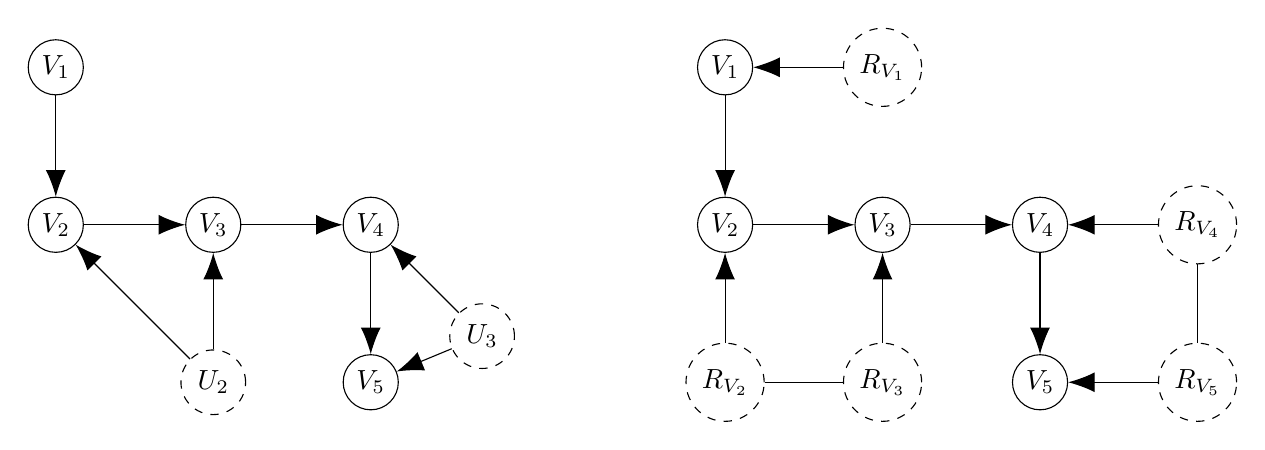
\begin{tikzpicture}[>=Stealth, node distance=2cm, on grid, auto]

  \begin{scope}
  \node (V1) [rv] {$V_1$};
  \node (V2) [below = of V1, rv] {$V_2$};
  \node (V3) [right = of V2, rv] {$V_3$};
  \node (V4) [right = of V3, rv] {$V_4$};
  \node (V5) [below = of V4, rv] {$V_5$};
  %\node (U1) [right = of V1] {$U_1$};
  \node[draw, circle, dashed] (U2) [below = of V3] {$U_2$};
  \node[draw, circle, dashed] (U3) [below right = of V4] {$U_3$};
  
  
  % Arrows
  \draw [-{Latex[scale=2.0]}] (V1) -- (V2);
  \draw [-{Latex[scale=2.0]}] (V2) -- (V3);
  \draw [-{Latex[scale=2.0]}] (V3) -- (V4);
%  \draw [-{Latex[scale=2.0]}] (V3) -- (V5);
  \draw [-{Latex[scale=2.0]}] (V4) -- (V5);
  
  % Dashed arrows (unobserved variables)
  %\draw [-{Latex[scale=2.0]}] (U1) -- (V1);
  \draw [-{Latex[scale=2.0]}] (U2) -- (V2);
  \draw [-{Latex[scale=2.0]}] (U2) -- (V3);
  \draw [-{Latex[scale=2.0]}] (U3) -- (V4);
  \draw [-{Latex[scale=2.0]}] (U3) -- (V5);
    
  \end{scope}% Nodes
  \begin{scope}[xshift=8.5cm]  % Nodes
  \node (V1) [rv] {$V_1$};
  \node (V2) [below = of V1, rv] {$V_2$};
  \node (V3) [right = of V2, rv] {$V_3$};
  \node (V4) [right = of V3, rv] {$V_4$};
  \node (V5) [below = of V4, rv] {$V_5$};
  \node[draw, circle, dashed] (RV1) [right = of V1] {$R_{V_1}$};
  \node[draw, circle, dashed] (RV2) [below = of V2] {$R_{V_2}$};
  \node[draw, circle, dashed] (RV3) [below = of V3] {$R_{V_3}$};
  \node[draw, circle, dashed] (RV4) [right = of V4] {$R_{V_4}$};
  \node[draw, circle, dashed] (RV5) [right = of V5] {$R_{V_5}$};
  
  % Arrows
  \draw [-{Latex[scale=2.0]}] (V1) -- (V2);
  \draw [-{Latex[scale=2.0]}] (V2) -- (V3);
  \draw [-{Latex[scale=2.0]}] (V3) -- (V4);
%  \draw [-{Latex[scale=2.0]}] (V3) -- (V5);
  \draw [-{Latex[scale=2.0]}] (V4) -- (V5);
  
  % Dashed arrows (unobserved variables)
  \draw [-{Latex[scale=2.0]}] (RV1) -- (V1);
  \draw [-{Latex[scale=2.0]}] (RV2) -- (V2);
  \draw [-{Latex[scale=2.0]}] (RV3) -- (V3);
  \draw [-{Latex[scale=2.0]}] (RV4) -- (V4);
  \draw [-{Latex[scale=2.0]}] (RV5) -- (V5);

  \draw[] (RV2) -- (RV3);
  \draw[] (RV4) -- (RV5);
\end{scope}
\end{tikzpicture}
\caption{A sequential instrumental variable example, and its response function variable transformation.\label{fig:seqiv}}
\end{figure}

\begin{remark} \label{rmk1}
Let $\mathcal{G}(\bV, \bU)$ be a hidden variables DAG that follows Conditions \ref{A1}, \ref{A2}, and has a c-degree of 1. The response variable transformation of $\mathcal{G}(\bV, \bU)$ results in the same structural model, i.e. the same values of all variables under any intervention (including no intervention) on any of the observed variables in the DAG. 
\end{remark}

The response function variable transformation preserves the marginal model, and also allows us to exploit the discreteness of the observations to formulate a set of linear constraints. Given a value of a response function variable, say $R_{V_i} = b$, there exists a response function $f_{V_i}^b(\Paobs(V_i))$ that determines an observed value for $V_i$ given $\Paobs(V_i)$. So $f_{V_i}^b: \operatorname{domain}(\Paobs(V_i)) \rightarrow \operatorname{domain}(V_i)$. Given values of the response function variables for $V_i$ and all of its ancestors, the value of $V_i$ is determined by recursive substitutions \citep{sachs2023general, duarte2023automated}. Therefore we can write all observable probabilities and interventional probabilities in terms of probabilities of response function variables. Following \citet{tian2002testable}, we will call the equations relating these two forms of probabilities \emph{functional constraints}. 


\subsection{Functional constraints}

An algorithm and implementation to obtain the set of functional constraints for DAGs that fit a more strict set of criteria than what we consider here was presented in Algorithm 1 of \citet{sachs2023general}. A more general algorithm for settings with arbitrary c-degree is presented in \citet{duarte2023automated}, where the constraints are polynomials. Their Proposition 4 states that the degree of the polynomial constraints is bounded above by the c-degree of the corresponding district. In our next Proposition we explicitly relate the functional constraints to observable probabilities, forming the foundation of the observable constraint derivation.



\begin{proposition} \label{prop:ident}
Suppose $\mathcal{G}(\bV, \bU)$ is a hidden variables DAG that follows Conditions \ref{A1} and \ref{A2}. Further, suppose $\bV_1$ is the vector of all observed variables in the district $D_1$, and let $\bV_2 = \Paobs(\bV_1) \setminus \bV_1$ be the vector of observed parents of $\bV_1$ that are not part of $\bV_1$. Order $\bV_1=(V_{11},\ldots,V_{1k})$ consistently with a topological ordering of $\mathcal{G}$, let $\bV_1^{<i}=(V_{11},\ldots,V_{1,i-1})$ and $\bV_1^{\leq i} = (V_{11},\ldots,V_{1i})$, and let
\[
\boldsymbol{C}_{i} = \bV_1^{<i} \cup \left\{\bV_2 \cap \Paobs(\bV_1^{\leq i})\right\},
\]
i.e., the earlier members of the district together with the external observed parents of $V_{1i}$ and of every earlier member. Writing $c_i$ for the corresponding subvector of $(v_1, v_2)$, define
\[
    \Pdo(\bV_1=v_1\mid \bV_2=v_2)
    =
    \prod_{i=1}^k
    \Pr\!\left(
        V_{1i}=v_{1i}
        \,\middle|\,
        \boldsymbol{C}_{i} = c_i
    \right).
\]
If $D_1$ has c-degree 1, then for all possible values of the vectors $v_1 = (v_{11}, \ldots, v_{1k}), v_2 = (v_{21}, \ldots, v_{2\ell})$, the functional constraints on $\Pdo(\bV_1 = v_{1} |\bV_2 = v_2)$ under $\mathcal{G}(\bV, \bU)$ are linear functions of response function variable probabilities of $\mathbf{R}_{\bV_1}$.
\end{proposition}

Under the conditional independencies implied by $\mathcal{G}$, conditioning additionally on any other variables that precede $V_{1i}$ in a topological ordering does not change the factor (see the proof of Proposition \ref{prop:ident}), but $\boldsymbol{C}_i$ cannot be made smaller in general.

Let $\Pr(\bV_1 = v_1 | \Do(\bV_2 = v_2))$ denote the joint probability of $\bV_1 = v_1$ under the intervention that sets $\bV_2 = v_2$. All of the $\Pdo(\bV_1 = v_{1} |\bV_2 = v_2)$ referenced in Proposition \ref{prop:ident} can be given a causal interpretation using the do operator, such that $\Pdo(\bV_1 = v_{1} |\bV_2 = v_2) =  \Pr(\bV_1 = v_{1} | \Do(\bV_2 = v_2))$. 

\begin{proposition} \label{causalprop}
Suppose $\mathcal{G}(\bV, \bU)$ is a hidden variables DAG that follows Conditions \ref{A1}, \ref{A2}, and $\bV_1$, $\bV_2$ are as described in Proposition \ref{prop:ident}. Then all $\Pr(\bV_1 = v_{1} | \Do(\bV_2 = v_2))$ are identified and given by $\Pdo(\bV_1 = v_1|\bV_2=v_2)$. 
\end{proposition}

Consider the example in Figure \ref{fig:ivclassic}, the left most of which is the classical IV setting. In this case there are 2 districts, $\{Z\}$ with c-degree 0 and $\{X, Y, U\}$ with c-degree 1, and Conditions \ref{A1} and \ref{A2} are satisfied. Letting $\bV_1 = (X, Y)$ and applying Proposition \ref{prop:ident} we have $\bV_2 = \Paobs(\{X, Y\}) \setminus \{X, Y\} = \{Z\}$, $\boldsymbol{C}_1 = \{Z\}$, $\boldsymbol{C}_2 = \{Z, X\}$, and
\begin{align*}
    \Pdo(\bV_1 = v_{1} |\bV_2 = v_2) &= \Pr(Y = y | X = x, Z = z) \Pr(X = x | Z = z)\\ 
    & = \Pr(X = x, Y = y | \Do(Z = z)) \\
    & = \sum_{b \in \mathcal{B}} \Pr((R_x, R_y) = b), \mbox{ for all } x, y, z,
\end{align*}
where $\mathcal{B} = \{(b_x, b_y): f^{b_y}_Y(f^{b_x}_X(z)) = y \mbox{ and } f^{b_x}_X(z) = x\}$ for the structural equations $f^{b_y}_Y$ and $f^{b_x}_X$. The series of functional constraints for each combination of values of $z, x, y$ can be represented by the matrix equation
\[
\boldsymbol{p_{xy\cdot z}} = \boldsymbol{B} \boldsymbol{r_{xy}}, 
\]
where, for binary $X, Y, Z$, $\boldsymbol{p_{xy\cdot z}}$ is the vector of 8 probabilities $[\Pr(Y = y | X = x, Z = z) \Pr(X = x | Z = z): x, y, z \in \{0, 1\}]$, $\boldsymbol{B}$ is an $8 \times 16$ matrix of 0s and 1s, and $\boldsymbol{r_{xy}}$ is the vector of 16 response function variable probabilities $[\Pr((R_x, R_y) = (b_x, b_y)): b_x, b_y \in \{0, 1, 2, 3\}]$.

\begin{figure}[ht]
\centering

    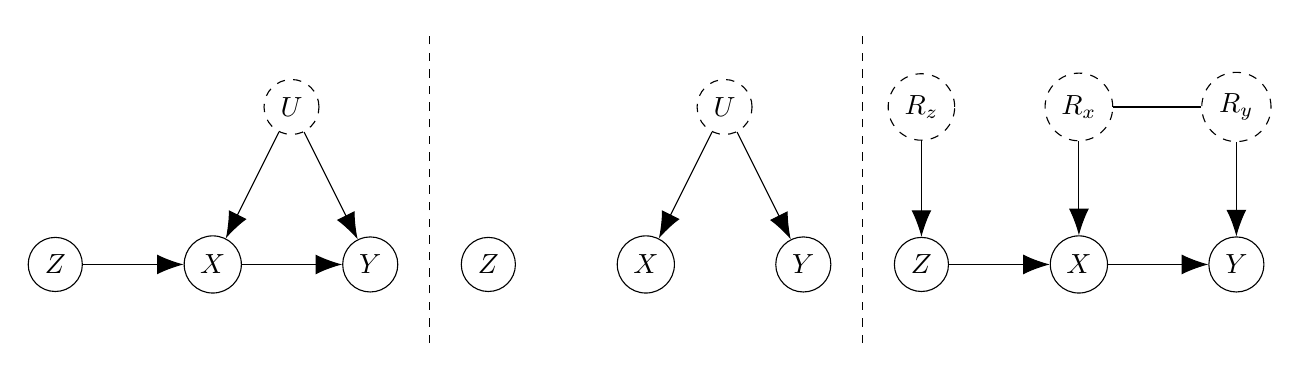
\begin{tikzpicture}
    \begin{scope}[xshift=-2cm]
    \node[draw, circle] at (2, 0) (X) {\(X\)};
    \node[draw, circle] at (4, 0) (Y) {\(Y\)};
    \node[draw, circle] at (0, 0) (Z) {$Z$};
    %\node[draw, circle] at (-3, 4) (S) {\(S\)};
   % \node[draw, circle] at (-4, 0) (Z) {\(Z\)};
    \node[draw, circle, dashed] at (3,2) (U) {\(U\)};
    \draw [-{Latex[scale=2.0]}] (X) to (Y);
    \draw [-{Latex[scale=2.0]}] (Z) to (X);
    %\draw [-{Latex[scale=2.0]}] (S) to (X);
    %\draw [-{Latex[scale=2.0]}] (S) to (Y);
    \draw [-{Latex[scale=2.0]}] (U) to (X);
    \draw [-{Latex[scale=2.0]}] (U) to (Y);
   % \draw [-{Latex[scale=2.0]}] (Z) to (X);
    %\draw [-, dashed] (S) to (U);
    \draw[dashed] (4.75, -1) -- (4.75, 3);

    \end{scope}% Nodes
\begin{scope}[xshift=3.5cm]
    \node[draw, circle] at (2, 0) (X) {\(X\)};
    \node[draw, circle] at (4, 0) (Y) {\(Y\)};
    \node[draw, circle] at (0, 0) (Z) {$Z$};
    %\node[draw, circle] at (-3, 4) (S) {\(S\)};
   % \node[draw, circle] at (-4, 0) (Z) {\(Z\)};
    \node[draw, circle, dashed] at (3,2) (U) {\(U\)};
  %  \draw [-{Latex[scale=2.0]}] (X) to (Y);
   % \draw [-{Latex[scale=2.0]}] (Z) to (X);
    %\draw [-{Latex[scale=2.0]}] (S) to (X);
    %\draw [-{Latex[scale=2.0]}] (S) to (Y);
    \draw [-{Latex[scale=2.0]}] (U) to (X);
    \draw [-{Latex[scale=2.0]}] (U) to (Y);
   % \draw [-{Latex[scale=2.0]}] (Z) to (X);
    %\draw [-, dashed] (S) to (U);
    \draw[dashed] (4.75, -1) -- (4.75, 3);

    \end{scope}% Nodes
    
  \begin{scope}[xshift=9cm] 
    
    \node[draw, circle] at (2, 0) (X) {\(X\)};
    \node[draw, circle] at (4, 0) (Y) {\(Y\)};
    \node[draw, circle] at (0, 0) (Z) {$Z$};
    %\node[draw, circle] at (-3, 4) (S) {\(S\)};
   % \node[draw, circle] at (-4, 0) (Z) {\(Z\)};
    \node[draw, circle, dashed] at (2,2) (Rx) {\(R_x\)};
    \node[draw, circle, dashed] at (4,2) (Ry) {\(R_y\)};
    \node[draw, circle, dashed] at (0,2) (Rz) {\(R_z\)};
    \draw [-{Latex[scale=2.0]}] (X) to (Y);
    \draw [-{Latex[scale=2.0]}] (Z) to (X);
    %\draw [-{Latex[scale=2.0]}] (S) to (X);
    %\draw [-{Latex[scale=2.0]}] (S) to (Y);
    \draw [-{Latex[scale=2.0]}] (Rx) to (X);
    \draw [-{Latex[scale=2.0]}] (Ry) to (Y);
    \draw [-{Latex[scale=2.0]}] (Rz) to (Z);
    \draw (Rx) -- (Ry);
   % \draw [-{Latex[scale=2.0]}] (Z) to (X);
    %\draw [-, dashed] (S) to (U);
  

  \end{scope}
    \end{tikzpicture}
  
    \caption{\label{fig:ivclassic} The instrumental variable DAG in original form (left), showing the two districts (center), and response variable form (right).}
    \end{figure}  

% Although we interpret the $\Pr(\bW_1 =w_1| \Do(\bW_2)=w_2)$ as causal, one does not need to do so. Instead, one can simply define $\Pr(\bW_1 =w_1| \Do(\bW_2)=w_2)$ to be a function that is given by:   
% \[
%     \prod_{i: W_{1i} \in D_1} \Pr(W_{1i} = w_{1i} | \{\Paobs(\bW_1) \cap \Anobs(W_{1i})\} \setminus W_{1i}).
% \]
% which allows one to equate $\Pr(\bW_1 =w_1| \Do(\bW_2)=w_2)$ with $Q_j$ in equation (29) of \citet{tian2002identification} without requiring a causal interpretation. The proof of Proposition \ref{prop:ident} then follows just as shown in the Appendix. 



\subsection{Nested Markov models} \label{sec:nested}

The nested Markov models \citep{richardson2023nested} further constrain the state-space of these sets of distributions. Briefly put, they allow (generalized) conditional independence constraints to be encoded within a hidden variables DAG model, and in the discrete case to know that these independences are the only \emph{equality} constraints in the model \citep{evans2018margins}. 


While a regular conditional independence relation, for example $X \indep Y \mid Z$, can be expressed as $\Pr(X | Y, Z) = \Pr(X | Z)$, a \emph{nested Markov independence} is a more general statement about a lack of dependence of a quantity on a particular variable. In particular, the quantities in question are probabilities in graphs after removing arrows into certain variables (i.e., intervening on them). For example, they can be expressed as $\sum_B \Pr(D | A, B, C)\Pr(B | A) = g(D, C)$, for some function $g$; note the lack of dependence on $A$ here. Such relations are also sometimes called \emph{Verma constraints} after \citet{verma2022equivalence}, and \emph{post-truncation independences} after \citet{shpitser2012parameter}.
Further details are given in the Appendix, Section \ref{sec:nmm}.

\subsection{Relation to previous work}

Our method combines three ingredients. These are the response function representation of \citet{balke1994counterfactual}, the V-to-H conversion that \citet{bonet2001instrumentality} applied to the instrumental variable model, and the district (c-component) factorization of \citet{tian2002identification, tian2002testable}. Each is known on its own. What is new is the following. First, we identify c-degree one as the class of graphs where every district factor is a linear image of a simplex, so the polytope argument applies one district at a time (Proposition \ref{prop:ident}). Second, we show that the district polytopes together with the ordinary conditional independencies are \emph{sufficient}, i.e., that nothing is lost when the joint distribution is reassembled from its district factors (Proposition \ref{prop:complete}). This step depends on the conditioning sets in Proposition \ref{prop:ident} being chosen correctly and on the ordered local Markov property. Third, we give an exact criterion for which constraints are nontrivial (Proposition \ref{prop:nontrivial}), and we use it to link the equality constraints to the nested Markov model. We also give a pre-processing step for graphs with higher c-degree and an open-source implementation. Our goal also differs from the related work of \citet{duarte2023automated}, who use the same response function polynomials to bound causal effects by optimization. We instead aim to list every restriction that the model places on the observed distribution, without reference to any target quantity.



\section{Method for deriving constraints and completeness results}

Given those preliminaries, we now detail our algorithm for deriving observable constraints in a hidden variables DAG with discrete and finite observed variables. To summarize briefly, we begin by using d-separation to list all conditional and marginal independencies implied by the DAG, if there are any. Then, for each district, we describe a convex polyhedron in terms of the probabilities of the response function variables and convert this to an equivalent description in terms of only observable quantities. This is called the vertex-to-halfspace (V-to-H) conversion, and different algorithms exist to efficiently perform this conversion that are implemented in open-source software programs such as \texttt{cddlib} \citep{cdd}.

\subsection{Description of the algorithm} \label{algorithm}


\textbf{Inputs: } A hidden variables DAG $\mathcal{G}(\bV, \bU)$ that meets Conditions \ref{A1}, \ref{A2} and has c-degree 1. 
\begin{enumerate}
    %\item Convert $\mathcal{G}'$ to the canonical DAG $\mathcal{G}$ using the Algorithm 1 of \citet{duarte2023automated}. 
   % \item Do the latent projection operation to get an ADMG $\mathcal{G}(\bV)$ \citep{verma2022equivalence}
    \item Enumerate the conditional independencies using a standard algorithm based on checking for d-separation, e.g., \citet{van2014constructing}, or using lines 1--8 of Algorithm 1 of \citet{richardson2023nested}.
    \item[] \, \textbf{Output: } List of standard independence constraints.  
    \item Identify the districts $\mathcal{D} = \{D_1, \ldots, D_M\}$. 
    \item Do the response function variable transformation of $\mathcal{G}$ into $\mathcal{G}(\bV, \bR)$ as described in Section \ref{sec:respvar}.
    \item For each district $D_j$: 
   \begin{enumerate}  
        \item Derive the formula for $\Pdo(\bV_1 = v_1 | \bV_2 = v_2)$, where $\bV_1$ are all the observed variables in $D_j$ and $\bV_2 = \Paobs(\bV_1) \setminus \bV_1$, using Proposition \ref{prop:ident}.
        \item For each combination of $v_1, v_2$, derive the functional probabilities, i.e., 
        \[
        \sum_{b \in \mathcal{B}} \Pr(\boldsymbol{R}_{\bV_1} = b), 
        \]
    where $\mathcal{B}$ is the set of response function variable values that are compatible with the observation vector $v_1, v_2$. 
    \item Construct the matrix representing the system of linear equations relating 
    \[
    \Pdo(\bV_1 = v_1 |\bV_2 = v_2) = \sum_{b \in \mathcal{B}} \Pr(\boldsymbol{R}_{\bV_1} = b) \Leftrightarrow \boldsymbol{p} = \boldsymbol{B} \boldsymbol{r}.
    \]
    \item Add a row of all 1s to $\boldsymbol{B}$ which represents the constraint that the response function variable probabilities all sum to 1. 
    \item Convert $\boldsymbol{p} = \boldsymbol{B} \boldsymbol{r}$ to the H-representation, e.g., using the double description method \citep{cdd, doubledescriptionmethod}.
    \item[] \, \textbf{Output: } The H-representation and the vector $\boldsymbol{p}$ of the formulae for $\Pdo(\bV_1 = v_1 |\bV_2 = v_2)$ for each district
    \end{enumerate}
\end{enumerate}

The H-representation consists of two rational matrices $H_i, H_e$ and rational vectors $b_i, b_e$ such that 
\[
H_i \boldsymbol{p} \leq b_i
\mbox{ and }
H_e \boldsymbol{p} = b_e. 
\]
In other words, it provides a representation of inequality and equality constraints in terms of the observable probability vector. 

We apply the Algorithm to the second district of the binary IV example which contains $X$ and $Y$. The worked details are in the Appendix, Section \ref{appendix:iv}. The equality constraints encoded by $H_e$ are simply the standard probabilistic constraints:
\begin{equation}
\sum_{x, y \in \{0, 1\}} \Pr(Y = y, X = x | Z = z) = 1, \mbox{ for } z = 0, 1. \label{eqn:ivex}
\end{equation}


\subsection{Completeness results} \label{sec:complete}



%\begin{definition}
%    A causal model $G$ is \emph{linear} if all distributions compatible with $G$ satisfy a linear system of functional constraints. 
%\end{definition}

%Thus, if a causal model is linear then the complete set of functional %constraints are linear. 

\begin{proposition} \label{prop:complete}
 Let $\mathcal{G}$ be a hidden variables DAG satisfying Conditions \ref{A1}, \ref{A2}, and having c-degree 1. Let $\mathcal{C}(\mathcal{G})$ be the set of observed distributions satisfying the conditional independencies implied by $\mathcal{G}$ and the district level H-representation constraints returned by the algorithm. Then
\[
    \mathcal{M}(\mathcal{G}) = \mathcal{C}(\mathcal{G}),
\]
where $\mathcal{M}(\mathcal{G})$ denotes the marginal model over the observed variables. Hence the constraints derived from the algorithm, together with the conditional independencies, are complete.
\end{proposition}

In other words, if every district in a DAG has at most one latent common cause, then the constraints derived by our algorithm are necessary and sufficient, i.e., the marginal model is exactly the set of observed distributions satisfying these constraints.


\begin{remark} \label{rmk:positivity}
Proposition \ref{prop:complete} extends to distributions with zero probabilities as follows. Order every district using one topological ordering of $\mathcal{G}$, and read each product in Proposition \ref{prop:ident} from $i = 1$ to $k$. The first factor that is not positive decides the entry of $\boldsymbol{p}$. If it is zero, the entry is zero, whatever follows it. If it is undefined, because $\Pr(\boldsymbol{C}_i = c_i) = 0$, the observed distribution does not determine the entry, and we treat the entry as a free variable. Then $\Pr \in \mathcal{M}(\mathcal{G})$ if and only if $\Pr$ satisfies the conditional independencies and, for each district, the free entries can be chosen so that $H_i \boldsymbol{p} \leq b_i$ and $H_e \boldsymbol{p} = b_e$. Equivalently, there is a probability vector $\boldsymbol{r}$ with $\boldsymbol{p} = \boldsymbol{B}\boldsymbol{r}$ on the remaining entries, which is a linear program. A strictly positive distribution has no free entries. The proof is in the Appendix.
\end{remark}

For example, in the instrumental variable model with $\Pr(Z = 1) = 0$, every entry with $z = 1$ is free, and $\Pr(x, y \mid Z = 0)$ is unrestricted. Free entries do not remove all restrictions, however. In the graph $A \rightarrow B \rightarrow C \rightarrow D$ with $U \rightarrow B$ and $U \rightarrow D$, if $C = B$ with probability one, the entries with $c \neq b$ are free, and the other entries must satisfy the instrumental inequalities for $(A, B, D)$. 

As a case where the Algorithm does not apply, consider the triangle scenario, in which three observed variables $A$, $B$, $C$ have no edges between them and each pair shares an unobserved parent. It has c-degree 3, and comprises a single district. Our algorithm cannot be applied in this case; however, it is known that some observed probability distributions are incompatible with the triangle scenario. For example, \citet{Wolfe_2019} demonstrates that the distribution where $\Pr(A = 1, B = 1, C = 1) = \Pr(A = 0, B = 0, C = 0) = 1/2$ is incompatible with the triangle scenario. An additional example is the left side of Figure \ref{fig:incomp}. As discussed in Section \ref{sec:nonlin} and \ref{graphmod}, one can modify such graphs to obtain some or all constraints in some settings. 



\subsection{Identifying nontrivial constraints} \label{sec:nontriv}

Not every constraint returned by the Algorithm restricts the observed distribution. The equality constraints include normalization, as in \eqref{eqn:ivex}, and the inequality constraints include nonnegativity, $\Pdo(\bV_1 = v_1 \mid \bV_2 = v_2) \geq 0$. Other equality constraints follow from the conditional independencies, which are listed separately in step 1 of the Algorithm, and other inequality constraints become nonnegativity constraints once equality constraints are added to them. Throughout this subsection, let $D$ be a district with observed members $\bV_1$ and external parents $\bV_2 = \Paobs(\bV_1) \setminus \bV_1$, write $p(v_1 \mid v_2) = \Pdo(\bV_1 = v_1 \mid \bV_2 = v_2)$ for the entries of the vector $\boldsymbol{p}$, and let $\boldsymbol{\check{P}}$ be the cross-product of probability simplices, one for each value of $v_2$. This is the set of vectors allowed by the standard probabilistic constraints alone.

\begin{definition} \label{def:nontrivial}
An equality constraint of $D$ is \textbf{trivial} if it holds for every strictly positive distribution of the observed variables that satisfies the conditional independencies implied by $\mathcal{G}$. An inequality constraint of $D$ is \textbf{trivial} if it holds for every $\boldsymbol{p} \in \boldsymbol{\check{P}}$ that satisfies the equality constraints of $D$. A constraint that is not trivial is \textbf{nontrivial}.
\end{definition}

The trivial equality constraints can be listed from the graph. Call a set $\bS \subseteq \bV_1$ \emph{closed} if it contains every member of $D$ that is an ancestor of a member of $\bS$. Equivalently, $\bS$ consists of the first members in some ordering of $\bV_1$ that is consistent with a topological ordering of $\mathcal{G}$. Let $\boldsymbol{E}(\bS) = \bV_2 \cap \Paobs(\bS)$ be the external parents of $\bS$. Consider the linear equations
\begin{itemize}
\item[(N)] $\sum_{v_1} p(v_1 \mid v_2) = 1$ for every $v_2$;
\item[(O)] for every nonempty closed set $\bS$, the margin $p_{\bS}(v_{\bS} \mid v_2) = \sum_{v_{\bV_1 \setminus \bS}} p(v_1 \mid v_2)$ takes the same value at any two values of $v_2$ that agree on $\boldsymbol{E}(\bS)$.
\end{itemize}
By Proposition \ref{causalprop}, $p_{\bS}(v_{\bS} \mid v_2)$ is the probability of $\bS = v_{\bS}$ under $\Do(\bV_2 = v_2)$, and (O) states that it does not depend on the external parents of the members outside $\bS$. We also write $N$ and $O$ for the coefficient matrices of these equations.

\begin{proposition} \label{prop:nontrivial}
Suppose $\mathcal{G}(\bV, \bU)$ is a hidden variables DAG that follows Conditions \ref{A1}, \ref{A2} and has c-degree 1. Let $H_i \boldsymbol{p} \leq b_i$, $H_e \boldsymbol{p} = b_e$ be the H-representation of a district $D$ returned by the Algorithm, in which each row of $H_i$ defines a different facet of the district polytope $\{\boldsymbol{B}\boldsymbol{r} : \boldsymbol{r} \text{ a probability vector}\}$ and the rows of $H_e$ define its affine hull. Then:
\begin{enumerate}
\item[(i)] An equality constraint $g^\top \boldsymbol{p} = d$ is trivial if and only if it is a linear combination of the equations (N) and (O). Hence the number of linearly independent nontrivial equality constraints of $D$ is
\[
\rank\begin{pmatrix} N \\ O \\ H_e \end{pmatrix} - \rank\begin{pmatrix} N \\ O \end{pmatrix},
\]
and any rows of $H_e$ that extend a basis of the rows of $(N; O)$ to a basis of the rows of $(N; O; H_e)$ imply, together with the conditional independencies, all equality constraints of $D$.
\item[(ii)] An inequality constraint $h^\top \boldsymbol{p} \leq c$ in $H_i$ is trivial if and only if some entry $p_k$ of $\boldsymbol{p}$ is zero at every column $\beta$ of $\boldsymbol{B}$ with $h^\top \beta = c$. In that case $c - h^\top \boldsymbol{p} = \alpha p_k + \lambda^\top (H_e \boldsymbol{p} - b_e)$ for some $\alpha > 0$ and vector $\lambda$, so the constraint is the nonnegativity constraint $p_k \geq 0$ written in a different form. If the constraint is nontrivial, then there is a strictly positive distribution of the observed variables that satisfies the conditional independencies and every constraint of every district except this one, which it violates.
\end{enumerate}
\end{proposition}

By Proposition \ref{prop:complete}, removing the trivial constraints from the output of the Algorithm does not change the model, and by part (ii), removing a nontrivial inequality constraint enlarges it. Part (ii) also shows that the trivial inequality constraints are exactly the nonnegativity constraints, possibly written in a different form. In (O), it is important to use every closed set, and not only the sets $\bV_1^{\leq i}$ of Proposition \ref{prop:ident}. For the sets $\bV_1^{\leq i}$, (O) holds for every strictly positive distribution, because $p_{\bV_1^{\leq i}}$ is the product of the first $i$ factors in Proposition \ref{prop:ident}. For the other closed sets, it is a consequence of the conditional independencies.

Both parts of Proposition \ref{prop:nontrivial} are exact and require no optimization. Part (i) needs only a few rank computations. Part (ii) needs only the incidence between facets and columns of $\boldsymbol{B}$: if $I$ is the 0/1 matrix with $I_{r\beta} = 1$ when column $\beta$ of $\boldsymbol{B}$ lies on the facet defined by row $r$ of $H_i$, then row $r$ is nontrivial if and only if every entry of row $r$ of $I \boldsymbol{B}^\top$ is positive. We compute $I$ in exact rational arithmetic.


The equations (O) are nested Markov constraints, and the nontrivial equality constraints of part (i) are Verma constraints. Call a set $\bS \subseteq \bV_1$ \emph{closed in the district} if it contains every member of $D$ that is a parent of a member of $\bS$. For such a set, the members of $\bS$ are functions of $v_{\boldsymbol{E}(\bS)}$ at every column of $\boldsymbol{B}$, so $p_{\bS}$ depends on $v_2$ only through its value on $\boldsymbol{E}(\bS)$, and this is an equality constraint of $D$. These are the constraints that the nested Markov model places on the district factor: $p_{\bS}$ is the kernel obtained by fixing the members outside $\bS$, and the constraint states that it does not depend on $\bV_2 \setminus \boldsymbol{E}(\bS)$ \citep{richardson2023nested}. When $\bS$ is closed, the constraint is of type (O), and by part (i) it is implied by the ordinary conditional independencies. A set can be closed in the district but not closed, because a member can be an ancestor of another member through variables outside $D$, and then the constraint is in general a Verma constraint. In the graph $A \rightarrow B \rightarrow C \rightarrow D$ with $U \rightarrow B$ and $U \rightarrow D$, for example, the district $\{B, D\}$ has external parents $\{A, C\}$, and the set $\{D\}$ is closed in the district but not closed. Its margin is
\[
\sum_b \Pdo(B = b, D = d \mid A = a, C = c) = \sum_b \Pr(b \mid a)\Pr(d \mid a, b, c),
\]
and the constraint states that it does not depend on $a$, as in the example of Section \ref{sec:nested}. With binary variables, these are the 2 nontrivial equality constraints that part (i) finds in this district. Since the nested Markov constraints are the only equality constraints of the marginal model \citep{evans2018margins}, every nontrivial equality constraint is a Verma constraint, and in all examples in this paper, the margin equations of the sets that are closed in the district but not closed span them.

Part (ii) must take the equality constraints into account. A row of $H_i$ is determined only up to a positive multiple and the addition of a linear combination of the rows of $H_e$, and which representative the double description method returns depends on its input. For example, in the graph $X \rightarrow A \leftarrow U \rightarrow B \leftarrow Y$ with binary variables, writing $p(ab \mid xy)$ for $\Pdo(A = a, B = b \mid X = x, Y = y)$, one of the returned rows is
\[
p(00 \mid 11) \leq p(00 \mid 10) + p(01 \mid 10).
\]
It is violated at points of $\boldsymbol{\check{P}}$ with $p(00 \mid 11) = 1$ and $p(00 \mid 10) = p(01 \mid 10) = 0$. But adding the equality constraint $p(00 \mid 10) + p(01 \mid 10) = p(00 \mid 11) + p(01 \mid 11)$, which is of type (O) with $\bS = \{A\}$, turns it into $p(01 \mid 11) \geq 0$. Accordingly, the 12 columns of $\boldsymbol{B}$ on its facet all have $p(01 \mid 11) = 0$. Of the 24 inequality constraints of this district, Proposition \ref{prop:nontrivial} identifies 8 as nontrivial, the CHSH inequalities \citep{clauser1969proposed}, and none of its 8 equality constraints are nontrivial.


Continuing with the IV example, the closed sets are $\{X\}$ and $\{X, Y\}$. Both have external parents $\{Z\}$, so (O) has no equations, and the two equality constraints \eqref{eqn:ivex} are the normalization constraints (N), which are trivial. Of the 12 inequality constraints, 8 are nonnegativity constraints. Proposition \ref{prop:nontrivial} identifies the other 4, the 2nd, 3rd, 5th and 6th rows of $H_i$ in the Appendix, Section \ref{appendix:iv}, as nontrivial. These are (after some simple algebra) the classical instrumental inequalities of \citet{pearl1995testability}:
\begin{align*}
 & \Pr(Y = 1,X = 1|Z = 0) + \Pr(Y = 0,X = 1|Z = 1) \leq 1 \\
& \Pr(Y = 0,X = 1|Z = 0) + \Pr(Y = 1,X = 1|Z = 1)  \leq 1 \\
& \Pr(Y = 1,X = 0|Z = 0) + \Pr(Y = 0,X = 0|Z = 1) \leq 1 \\
& \Pr(Y = 0,X = 0|Z = 0) + \Pr(Y = 1,X = 0|Z = 1) \leq 1.
\end{align*}
Singleton districts with no parents, such as $\{Z\}$, have only the trivial constraints (N) and nonnegativity. The sequential instrumental variable model of Figure \ref{fig:seqiv} has the conditional independence $(V_1, V_2) \indep (V_4, V_5) \mid V_3$ and two sets of these inequalities, one for each of the districts $\{V_2, V_3\}$ and $\{V_4, V_5\}$.

The front door model $A \rightarrow M \rightarrow Y$ with $U \rightarrow A$ and $U \rightarrow Y$ is known to have no nontrivial constraints \citep{pearl1995testability}. Its district $\{A, Y\}$ has external parent $M$. The closed sets are $\{A\}$, because $A$ is an ancestor of $Y$ through $M$, and $\{A, Y\}$. For $\bS = \{A\}$, (O) states that $\sum_y \Pdo(A = a, Y = y \mid M = m)$ does not depend on $m$, which in observed probabilities reads $\Pr(A = a) = \Pr(A = a)$. Together with normalization, these equations account for all 3 equality constraints of the district, so none of them is nontrivial. Each of the 8 inequality constraints is a nonnegativity constraint, so Proposition \ref{prop:nontrivial} correctly finds no nontrivial constraints.


\section{Novel Examples}
\subsection{Nested equivalent models with distinct inequalities}

\begin{figure}[ht]
    \centering
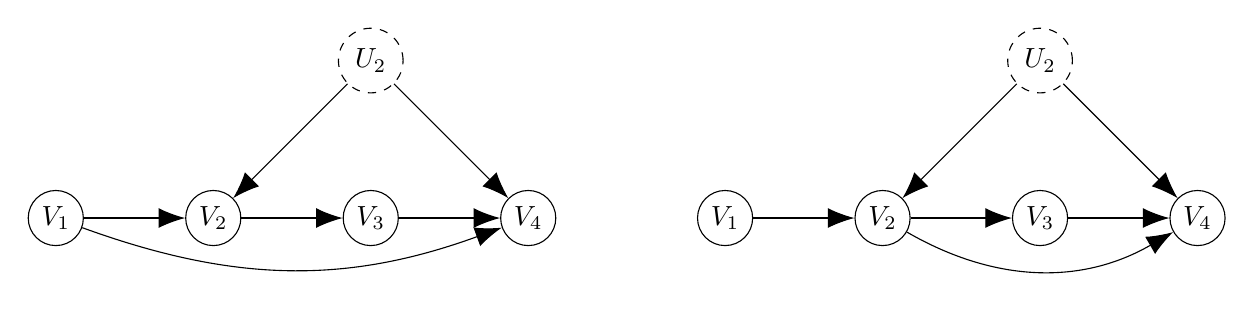
\begin{tikzpicture}[>=Stealth, node distance=2cm, on grid, auto]
  % Nodes
  \begin{scope}
  \node (V1) [rv] {$V_1$};
  \node (V2) [right = of V1, rv] {$V_2$};
  \node (V3) [right = of V2, rv] {$V_3$};
  \node (V4) [right = of V3, rv] {$V_4$};
  % \node (V5) [below = of V2, rv, xshift=10mm, yshift=3mm] {$V_5$};
  %\node (U1) [right = of V1] {$U_1$};
  % \node (U1) [right = of V5] {$U_1$};
  \node[draw,circle,dashed] (U2) [above = of V3] {$U_2$};
  
  
  % Arrows
  \draw [-{Latex[scale=2.0]}] (V1) -- (V2);
  \draw [-{Latex[scale=2.0]}] (V2) -- (V3);
  \draw [-{Latex[scale=2.0]}] (V3) -- (V4);
  % \draw [-{Latex[scale=2.0]}] (V1) -- (V5);
  \draw [-{Latex[scale=2.0]}] (V1) to[bend right=20] (V4);
  
  % Dashed arrows (unobserved variables)
  %\draw [-{Latex[scale=2.0]}] (U1) -- (V1);
  % \draw [-{Latex[scale=2.0]}] (U1) -- (V5);
  % \draw [-{Latex[scale=2.0]}] (U1) -- (V4);
  \draw [-{Latex[scale=2.0]}] (U2) -- (V4);
  \draw [-{Latex[scale=2.0]}] (U2) -- (V2);
\end{scope}
    

    \begin{scope}[xshift=8.5cm]
  \node (V1) [rv] {$V_1$};
  \node (V2) [right = of V1, rv] {$V_2$};
  \node (V3) [right = of V2, rv] {$V_3$};
  \node (V4) [right = of V3, rv] {$V_4$};
  % \node (V5) [below = of V2, rv, xshift=10mm, yshift=3mm] {$V_5$};
  %\node (U1) [right = of V1] {$U_1$};
  % \node (U1) [right = of V5] {$U_1$};
  \node[draw,circle,dashed] (U2) [above = of V3] {$U_2$};
  
  
  % Arrows
  \draw [-{Latex[scale=2.0]}] (V1) -- (V2);
  \draw [-{Latex[scale=2.0]}] (V2) -- (V3);
  \draw [-{Latex[scale=2.0]}] (V3) -- (V4);
  % \draw [-{Latex[scale=2.0]}] (V5) -- (V4);
  % \draw [-{Latex[scale=2.0]}] (V1) -- (V5);
  \draw [-{Latex[scale=2.0]}] (V2) to[bend right] (V4);

  % Dashed arrows (unobserved variables)
  %\draw [-{Latex[scale=2.0]}] (U1) -- (V1);
  % \draw [-{Latex[scale=2.0]}] (U1) -- (V5);
  % \draw [-{Latex[scale=2.0]}] (U1) -- (V4);
  \draw [-{Latex[scale=2.0]}] (U2) -- (V4);
  \draw [-{Latex[scale=2.0]}] (U2) -- (V2);
\end{scope}
\end{tikzpicture}
    \caption{Two graphs that are nested Markov equivalent, but which have distinct inequality constraints.}
    \label{fig:nested-ineq}
\end{figure}

Figure \ref{fig:nested-ineq} shows two graphs that have the same equality constraints, and hence the same nested Markov model, but different inequality constraints. Both graphs satisfy Conditions \ref{A1} and \ref{A2}, have c-degree 1, and have the districts $\{V_1\}$, $\{V_2, V_4, U_2\}$ and $\{V_3\}$, of which $\{V_1\}$ and $\{V_3\}$ have only trivial constraints. Both graphs imply $V_1 \indep V_3 \mid V_2$, and in both the district $\{V_2, V_4, U_2\}$ has the factor
\begin{align*}
& \Pdo(V_2 = v_2, V_4 = v_4 \mid V_1 = v_1, V_3 = v_3) \\
& \quad = \Pr(V_2 = v_2 \mid V_1 = v_1) \Pr(V_4 = v_4 \mid V_2 = v_2, V_1 = v_1, V_3 = v_3).
\end{align*}
Its 6 equality constraints are the same in both graphs. By Proposition \ref{prop:nontrivial}(i) they are all trivial: they are normalization and (O) with $\bS = \{V_2\}$, which this factorization satisfies identically. So the conditional independence is the only equality constraint of either graph.

The 16 inequality constraints of the left graph are all nonnegativity constraints, so it has no other restrictions. In the right graph, Proposition \ref{prop:nontrivial}(ii) identifies 8 of the 24 inequality constraints as nontrivial, and the other 16 are nonnegativity constraints. With binary variables, and after adding equality constraints to some of the rows returned by the Algorithm, the 8 nontrivial constraints are
\begin{equation}
\Pdo(V_2 = v_2, V_4 = v_4 \mid V_1 = 0, V_3 = v_3) + \Pdo(V_2 = v_2, V_4 = 1 - v_4 \mid V_1 = 1, V_3 = v_3) \leq 1, \label{eqn:nestedineq}
\end{equation}
for $v_2, v_3, v_4 \in \{0, 1\}$. For each value of $v_3$, these are the instrumental inequalities of \citet{pearl1995testability}, with instrument $V_1$, treatment $V_2$ and outcome $V_4$.

The inequalities \eqref{eqn:nestedineq} express that $V_1$ affects $V_4$ only through $V_2$ and $V_3$. In the right graph, the potential outcome $V_4(v_2, v_3)$ does not depend on $v_1$, so the left side of \eqref{eqn:nestedineq} is
\[
\Pr(V_2(0) = v_2, V_4(v_2, v_3) = v_4) + \Pr(V_2(1) = v_2, V_4(v_2, v_3) = 1 - v_4).
\]
These two events are mutually exclusive, because they require the same potential outcome to take different values. So the sum is at most 1. A violation rules out the right graph, and is what we would expect if $V_1$ changes $V_4$ with $V_2$ and $V_3$ held fixed, as the edge $V_1 \rightarrow V_4$ in the left graph allows. The left graph also has an exclusion restriction, because $V_2$ affects $V_4$ only through $V_3$. But it has no observable consequences beyond the conditional independence: given $V_1$, the unobserved $U_2$ can determine $V_2$, so $V_4$ can depend on $V_2$ through $V_1$ and $U_2$.

\subsection{Tripartite Bell graphs} \label{sec:tripart}

\begin{figure}[ht]
\begin{center}
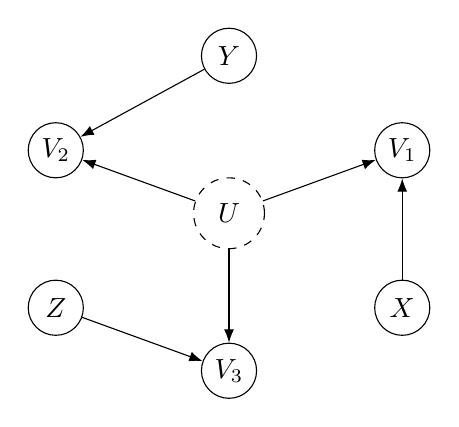
\begin{tikzpicture}[
    >=Latex,
    var/.style   ={draw,circle,minimum size=9mm,inner sep=0pt},
    latent/.style={draw,dashed,circle,minimum size=9mm,inner sep=0pt}
]
% Nodes (top row: X Y Z; bottom row: A B C; latent U centered above)
\node[latent]  (L) at (0,0)    {$U$};

\node[rv] (A) at ( 2.2, 0.8) {$V_1$};
\node[rv] (X) at ( 2.2,-1.2) {$X$};

\node[rv] (C) at ( 0.0,-2.0) {$V_3$};
\node[rv] (Z) at (-2.2,-1.2) {$Z$};

\node[rv] (B) at (-2.2, 0.8) {$V_2$};
\node[rv] (Y) at ( 0.0, 2.0) {$Y$};

% Arrows from settings to outcomes
\draw[->] (X) -- (A);
\draw[->] (Y) -- (B);
\draw[->] (Z) -- (C);

% Arrows from latent to outcomes
\draw[->] (L) -- (A);
\draw[->] (L) -- (B);
\draw[->] (L) -- (C);

\end{tikzpicture}
\end{center}
\caption{The tripartite Bell scenario. \label{fig:tripart}}
\end{figure}

Figure \ref{fig:tripart} is a well-known causal model in quantum physics. An incomplete set of constraints has been derived using the entropy method in \citet{bell3}. Our algorithm finds the complete set of constraints in this setting in about 19 minutes (Table \ref{tab:compute}). First we identify the standard independencies $X \indep (V_2, V_3, Y, Z)$, $Y \indep (V_1, V_3, X, Z)$, and $Z \indep (V_1, V_2, X, Y)$. The subsequent part of the algorithm yields an additional 53,894 constraints total, out of which there are 53,856 inequality constraints, in agreement with \citet{Sliwa2003Symmetries} and \citet{Pironio_2011}. Proposition \ref{prop:nontrivial} identifies 53,792 of the inequality constraints as nontrivial; the other 64 are nonnegativity constraints. None of the 38 equality constraints is nontrivial. Besides normalization, they are of type (O) and follow from the independence relations above: they state that the distribution of any two of $V_1, V_2, V_3$ does not depend on the setting of the third party, as in $(V_1, V_3) \indep Y \mid X, Z$, $(V_1, V_2) \indep Z \mid X, Y$, and $(V_2, V_3) \indep X \mid Y, Z$. An example of one of the inequality constraints, using the notation $\Pr(v_1 v_2 v_3 | xyz) = \Pr(V_1 = v_1, V_2 = v_2, V_3 = v_3 | X = x, Y = y, Z = z)$, is

\begin{align*}
& \Pr(001|010) + \Pr(010|101) - \Pr(110|001) - \Pr(010|100) - \\
& \Pr(000|111) - \Pr(001|000) - \Pr(011|000) \leq 0.
\end{align*}
Here the district factor of Proposition \ref{prop:ident} is $\Pr(v_1 \mid x)\Pr(v_2 \mid v_1, x, y)\Pr(v_3 \mid v_1, v_2, x, y, z) = \Pr(v_1 v_2 v_3 \mid xyz)$ under these independencies.


\subsection{Graphical structures that imply inequality constraints} \label{sec:structures}

The examples in this section and in Section \ref{sec:nontriv} have nontrivial inequality constraints in some districts and none in others. For a district of c-degree one, two structures in the graph guarantee nontrivial inequality constraints. Let $D$ be a district of c-degree one, with observed members $\bV_1$ and external parents $\bV_2 = \Paobs(\bV_1) \setminus \bV_1$. Say that an external parent $W \in \bV_2$ \emph{reaches} a member $V$ if there is a directed path from $W$ to $V$ all of whose vertices other than $W$ are members of $D$.

\begin{remark} \label{prop:ineqstructure}
Let $\mathcal{G}$ satisfy Conditions \ref{A1} and \ref{A2} and have c-degree one, and let $D$ be a district of $\mathcal{G}$ whose observed members and external parents each have at least two levels, and that contains at least one of the following:
\begin{enumerate}
\item[(i)] (\emph{instrumental type}) members $A$ and $B$, with $A$ a parent of $B$, and a directed path from some $W \in \bV_2$ to $A$, all of whose vertices other than $W$ are members of $D$, such that no vertex on the path other than $A$ is a parent of $B$;
\item[(ii)] (\emph{Bell type}) members $A$ and $B$ and external parents $W_A, W_B \in \bV_2$ such that $W_A$ reaches $A$ but not $B$, and $W_B$ reaches $B$ but not $A$.
\end{enumerate}
Then the H-representation of $D$ contains a nontrivial inequality constraint. Hence, by Proposition \ref{prop:nontrivial}(ii), there is a strictly positive distribution of the observed variables that satisfies the conditional independencies and every constraint of every district except this one, which it violates.
\end{remark}

The proof is in Appendix \ref{appendix:proofs}.

In both types, the inequality constraints come from exclusion restrictions. In type (i), $W$ and the members on the path to $A$ are excluded from $B$, so $W$ acts as an instrument for the effect of $A$ on $B$. In type (ii), $W_A$ is excluded from $B$ and $W_B$ from $A$. Type (i) appears in the instrumental variable model, in both districts of Figure \ref{fig:seqiv}, and in the right graph of Figure \ref{fig:nested-ineq}, with $(W, A, B) = (V_1, V_2, V_4)$. Type (ii) appears in the tripartite Bell district, in $X \rightarrow A \leftarrow U \rightarrow B \leftarrow Y$, and in the district $\{B, D\}$ of $A \rightarrow B \rightarrow C \rightarrow D$ with $U \rightarrow B$ and $U \rightarrow D$. The merged second district of Figure \ref{fig:incomp} contains both. The districts in our examples without nontrivial inequality constraints contain neither: the front door model, the left graph of Figure \ref{fig:nested-ineq}, and the first district of Figure \ref{fig:incomp}. Because graphs related by Proposition \ref{prop:hlp} have the same constraints, the conclusion also holds if the structure appears only after edges are added or removed using that proposition.

Remark \ref{prop:ineqstructure} gives a sufficient condition only, and these mechanisms are known. Whether a graph implies any inequality constraints at all has been studied for hidden variable DAGs in general. \citet{evans2023latent} shows that a discrete hidden variable DAG implies no nontrivial inequality constraints if and only if its marginal model is that of a DAG without hidden variables, and gives the CHSH inequalities of the district $\{B, D\}$ above as an example. \citet{khanna2024classifying} use this result, together with d-separation, e-separation and incompatible supports, to classify graphs with up to four observed variables, leaving 3 of the 2809 graphs with four observed variables unresolved. Graphs with a structure of type (i) are covered by their result on nonmaximal graphs: $W$ and $B$ are not adjacent, and they cannot be d-separated, because conditioning on a member on the path from $W$ to $B$ opens a path through the shared unobserved variable. In the other direction, if edges can be added using Proposition \ref{prop:hlp} until the unobserved variables can be removed without changing the conditional independencies, then the graph implies no inequality constraints \citep{henson2014theory}. Whether this criterion is also necessary is the conjecture discussed by \citet{khanna2024classifying}, which is open in general.

Remark \ref{prop:ineqstructure} is also related to the e-separation criterion of \citet{evans2012graphical}. Sets $A$ and $B$ are e-separated given $C$ after deleting $D$ if they are d-separated given $C$ in the graph with the nodes in $D$ removed. If, in addition, no vertex in $C$ is a descendant of a vertex in $D$, then for each value $d$ of $D$, the probabilities $\Pr(a, b, d \mid c)$ must be compatible with a distribution in which $A \indep B \mid C$ \citep[Theorem 4.2]{evans2012graphical}. This is often an inequality constraint \citep{evans2012graphical, finkelstein2021entropic}, but it need not be a new constraint: in the left graph of Figure \ref{fig:nested-ineq}, $V_1$ and $V_3$ are e-separated after deleting $V_2$, which only restates $V_1 \indep V_3 \mid V_2$. e-separation applies to graphs of any c-degree, but it gives only a sufficient condition, and it detects inequality constraints of the instrumental type: in the instrumental variable model, $Z$ and $Y$ are e-separated after deleting $X$, which yields the instrumental inequality, and in the right graph of Figure \ref{fig:nested-ineq}, $V_1$ and $V_4$ are e-separated after deleting $\{V_2, V_3\}$. It does not detect those of the Bell type: \citet[Remark 2.6]{evans2023latent} notes that the CHSH inequality cannot be read off in this way. In the graph $X \rightarrow A \leftarrow U \rightarrow B \leftarrow Y$, for example, $A$ and $B$ share the unobserved $U$, which cannot be deleted, while the pairs that can be separated, such as $X$ and $B$, are marginally independent, which yields only that independence. Remark \ref{prop:ineqstructure} is restricted to districts of c-degree one but covers both types. It identifies structures that produce inequality constraints, but not which inequalities arise. These form many families; for example, instrumental-type districts acquire new inequalities when the instrument has three or more levels \citep{bonet2001instrumentality}.


\section{Graphs with c-degree greater than one}
\label{sec:nonlin}
We extend our Algorithm to DAGs with c-degree greater than 1 that cannot be reduced to c-degree 1 using the rules of Section \ref{graphmod}. Prior to applying the Algorithm in Section \ref{algorithm}, for each district with c-degree at least 2, we replace all its unobserved variables by a single unobserved parent of every member that had an unobserved parent.

\begin{remark}
\label{prop:merge}
Let $\mathcal{G}'$ be a DAG satisfying Conditions \ref{A1}, \ref{A2}, and with c-degree greater than 1. Let $\mathcal{G}$ be the causal model obtained from $\mathcal{G}'$ by merging unobserved variables so that the c-degree is 1. 
Then the constraints admitted by $\mathcal{G}$ hold under $\mathcal{G}'$.
\end{remark}

Step 1 of the Algorithm should still be applied to $\mathcal{G}'$, because merging can remove conditional independencies.

We now consider the two examples where our algorithm does not apply as discussed in Section \ref{sec:complete}.
Figure \ref{fig:incomp}, left side, shows an example DAG that also appears in  \citet{duarte2023automated}. This DAG has two districts, $\{V_1, V_3, V_6, U_2\}$ that has c-degree 1 and $\{V_2, V_4, V_5, U_1, U_3\}$ that has c-degree 2. It satisfies Conditions \ref{A1} and \ref{A2}, but since the c-degree is greater than 1, we cannot guarantee that the constraints derived by our algorithm are complete. In this case, we proceed by merging the unobserved variables $U_1$ and $U_3$ into a single unobserved variable $U_{13}$ that has child set equal to the union of the child sets of $U_1$ and $U_3$ (Figure \ref{fig:incomp}, right side).


\begin{figure}[ht]
\begin{center}
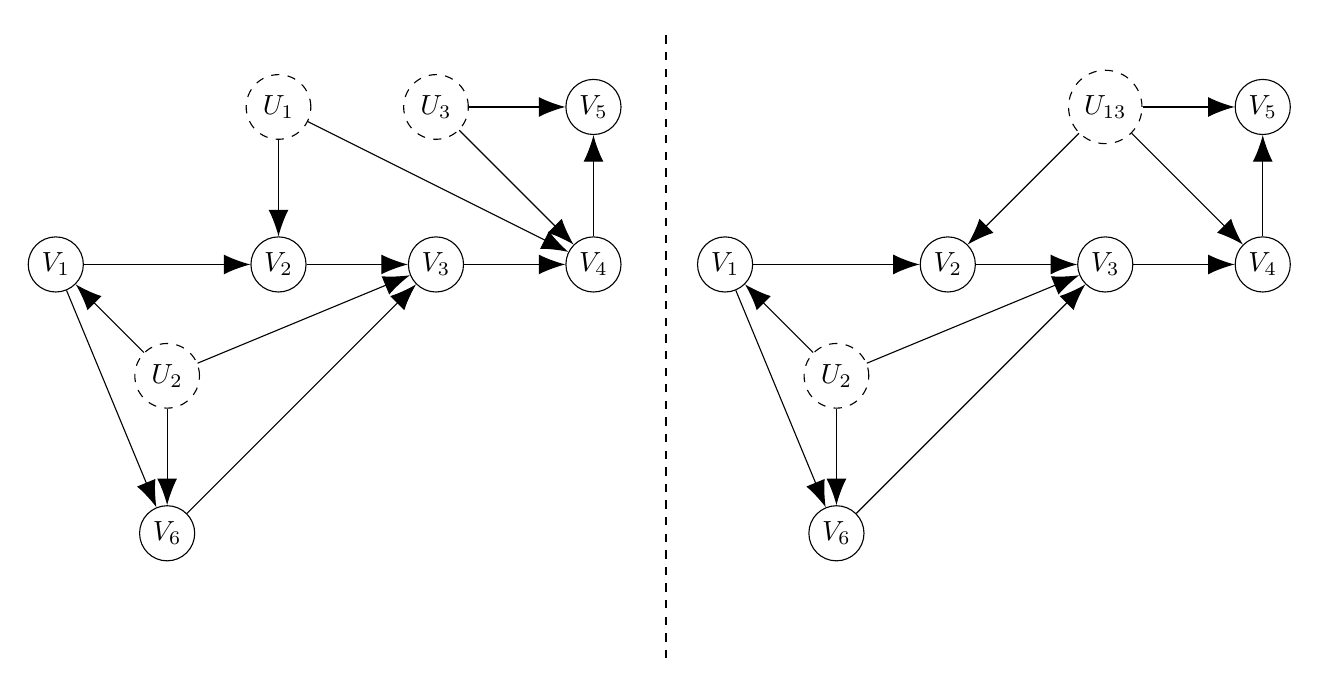
\begin{tikzpicture}[>=Stealth, node distance=2cm, on grid, auto]
\begin{scope}
  % Nodes
  \node (A) [rv] {$V_1$};
  \node[draw,circle,dashed] (U2) [below right= of A] {$U_2$};
  \node (B) [above right=of U2, rv] {$V_2$};
  \node (C) [right=of B, rv] {$V_3$};
  \node (D) [right=of C, rv] {$V_4$};
  
  \node (F) [above =of D, rv] {$V_5$};

  % unobserved variables (U1, U2, U3)
  \node[draw,circle,dashed] (U1) [above =of B] {$U_1$};
  
  \node[draw,circle,dashed] (U3) [above =of C] {$U_3$};
\node (E) [below=of U2, rv] {$V_6$};
  % Arrows
  \draw [-{Latex[scale=2.0]}]  (A) -- (B);
  \draw [-{Latex[scale=2.0]}]  (E) -- (C);
  \draw [-{Latex[scale=2.0]}]  (C) -- (D);
  \draw [-{Latex[scale=2.0]}]  (D) -- (F);
  \draw [-{Latex[scale=2.0]}]  (A) -- (E);
  \draw [-{Latex[scale=2.0]}]  (B) -- (C);

  % Dashed arrows (unobserved variables)
  \draw [-{Latex[scale=2.0]}] (U1) -- (B);
  \draw [-{Latex[scale=2.0]}] (U1) -- (D);
  \draw [-{Latex[scale=2.0]}] (U2) -- (A);
  \draw [-{Latex[scale=2.0]}] (U2) -- (E);
  \draw [-{Latex[scale=2.0]}] (U2) -- (C);
  \draw [-{Latex[scale=2.0]}] (U3) -- (F);
  \draw [-{Latex[scale=2.0]}] (U3) -- (D);
   \draw[dashed] (7.75, -5) -- (7.75, 3);
\end{scope}
\begin{scope}[xshift=8.5cm]
  \node (A) [rv] {$V_1$};
  \node[draw,circle,dashed] (U2) [below right= of A] {$U_2$};
  \node (B) [above right=of U2, rv] {$V_2$};
  \node (C) [right=of B, rv] {$V_3$};
  \node (D) [right=of C, rv] {$V_4$};
  
  \node (F) [above =of D, rv] {$V_5$};

  % unobserved variables (U1, U2, U3)
  %\node[draw,circle,dashed] (U1) [above =of B] {$U_1$};
  
  \node[draw,circle,dashed] (U13) [above =of C] {$U_{13}$};
\node (E) [below=of U2, rv] {$V_6$};
  % Arrows
  \draw [-{Latex[scale=2.0]}]  (A) -- (B);
  \draw [-{Latex[scale=2.0]}]  (E) -- (C);
  \draw [-{Latex[scale=2.0]}]  (C) -- (D);
  \draw [-{Latex[scale=2.0]}]  (D) -- (F);
  \draw [-{Latex[scale=2.0]}]  (A) -- (E);
  \draw [-{Latex[scale=2.0]}]  (B) -- (C);

  % Dashed arrows (unobserved variables)
  \draw [-{Latex[scale=2.0]}] (U13) -- (B);
  \draw [-{Latex[scale=2.0]}] (U13) -- (D);
  \draw [-{Latex[scale=2.0]}] (U2) -- (A);
  \draw [-{Latex[scale=2.0]}] (U2) -- (E);
  \draw [-{Latex[scale=2.0]}] (U2) -- (C);
  \draw [-{Latex[scale=2.0]}] (U13) -- (F);
\end{scope}
\end{tikzpicture}
\end{center}
\caption{Example model with two districts and c-degree 2 (left side), and the model after merging the unobserved variables $U_1$ and $U_3$ to make the c-degree 1 (right side). \label{fig:incomp}}
\end{figure}

For the first district in the graph in Figure \ref{fig:incomp} that contains $V_1, V_3, V_6$, Proposition \ref{prop:nontrivial} finds no nontrivial constraints. Besides normalization, the equality constraints are
\[
\Pdo(V_1 = v_1, V_6 = v_6 \mid V_2 = 0) = \Pdo(V_1 = v_1, V_6 = v_6 \mid V_2 = 1), \quad v_1, v_6 \in \{0, 1\},
\]
which are of type (O) with $\bS = \{V_1, V_6\}$. The district factor is $\Pdo(v_1, v_3, v_6 \mid v_2) = \Pr(v_1)\Pr(v_6 \mid v_1)\Pr(v_3 \mid v_1, v_6, v_2)$, so $\Pdo(v_1, v_6 \mid v_2) = \Pr(v_1, v_6)$. The equalities therefore hold identically, and the inequalities reduce to nonnegativity.


After merging $U_1$ and $U_3$ in the second district and applying our algorithm, Proposition \ref{prop:nontrivial} identifies 1096 nontrivial inequality constraints and 6 linearly independent nontrivial equality constraints. The district factor is
\[
\Pdo(v_2, v_4, v_5 \mid v_1, v_3) = \Pr(v_2 \mid v_1)\Pr(v_4 \mid v_1, v_2, v_3)\Pr(v_5 \mid v_1, v_2, v_3, v_4).
\]
Under $\Do(V_1 = v_1, V_3 = v_3)$, the variable $V_2$ depends only on $v_1$ and $U_{13}$, and $V_4$ depends only on $v_3$ and $U_{13}$. Since $V_2$ reaches $(V_4, V_5)$ only through $V_3$, which is held fixed, the equality constraints include the condition that $\sum_{v_2}\Pdo(v_2, v_4, v_5 \mid v_1, v_3)$ does not depend on $v_1$. In observed terms this reads
\[
\sum_{v_2} \Pr(v_2 \mid v_1)\Pr(v_4, v_5 \mid v_1, v_2, v_3) \mbox{ does not depend on } v_1,
\]
which is a Verma-type constraint, and which a randomly chosen distribution violates. Together with the trivial equality constraints, this condition implies all 6 nontrivial equality constraints of the district. The set $\{V_4, V_5\}$ is closed in the district but not closed, because $V_2$ is an ancestor of $V_4$ through $V_3$, as in Section \ref{sec:nontriv}. The inequality constraints imply
\begin{equation}
\sum_{v_1, v_3 \in \{0,1\}} \; \sum_{v_2, v_4, v_5 \in \{0,1\}} a(v_1, v_2, v_3, v_4) \, \Pdo(v_2, v_4, v_5 \mid v_1, v_3) \leq 3, \label{eqn:chsh}
\end{equation}
where $a(v_1, v_2, v_3, v_4) = (1 - v_1 v_3)\,\mathbf{1}\{v_2 = v_4\} + v_1 v_3\,\mathbf{1}\{v_2 \neq v_4\}$ and $\mathbf{1}\{\cdot\}$ is the indicator function. Thus $a = 1$ if $V_2$ and $V_4$ are equal when $v_1 v_3 = 0$, or differ when $v_1 = v_3 = 1$, and $a = 0$ otherwise. For each $(v_1, v_3)$, the inner sum in \eqref{eqn:chsh} is the probability of this event under $\Do(V_1 = v_1, V_3 = v_3)$. The inequality states that these four probabilities sum to at most 3. This is a Bell-type inequality. To see that it is nontrivial, consider the following distribution of binary variables:
\begin{itemize}
    \item $\Pr(V_1 = 1) = 1/2$, and $\Pr(V_2 = 1 \mid v_1) = \Pr(V_6 = 1 \mid v_1) = \Pr(V_3 = 1 \mid v_1, v_6, v_2) = \Pr(V_5 = 1 \mid v_1, v_2, v_3, v_4) = 1/2$ for all values of the conditioning variables;
    \item $\Pr(V_4 = v_4 \mid v_1, v_2, v_3) = 1/8 + \frac{3}{4}\, a(v_1, v_2, v_3, v_4)$, that is, $7/8$ if $a(v_1, v_2, v_3, v_4) = 1$ and $1/8$ otherwise.
\end{itemize}
Every probability in the resulting joint distribution of $(V_1, \ldots, V_6)$ is at least $1/256$. The distribution satisfies all the conditional independencies and all the equality constraints of both districts; in particular, $\Pdo(V_4 = 1 \mid v_1, v_3) = 1/2$ for all $v_1, v_3$. Yet for each of the four values of $(v_1, v_3)$, the inner sum in \eqref{eqn:chsh} equals $7/8$, so the left side equals $7/2 > 3$. By Remark \ref{prop:merge}, this distribution is therefore also incompatible with the original graph in Figure \ref{fig:incomp}, left. Given any observed distribution, it is straightforward to check the remaining constraints using the matrix representations returned by the software. The example distribution violates 13 of the inequality constraints returned for this district. The shortest of them is
\begin{align*}
\Pdo(V_2 = 0, V_4 = 1, V_5 = 0 \mid V_1 = 1, V_3 = 1) \leq{} & \Pdo(V_2 = 1, V_4 = 0 \mid V_1 = 0, V_3 = 0) \\
& + \Pdo(V_2 = 0, V_4 = 1, V_5 = 0 \mid V_1 = 1, V_3 = 0) \\
& + \Pdo(V_2 = 0, V_4 = 1, V_5 = 0 \mid V_1 = 0, V_3 = 1).
\end{align*}
For the example distribution, the left side equals $7/32$ and the right side equals $1/16 + 1/32 + 1/32 = 1/8$, so the constraint is violated.

For the triangle scenario, merging the three unobserved variables gives a single common parent of all three observed variables, which has no nontrivial constraints. So the constraints are incomplete in this case, because of the nontrivial constraints presented in \citet{Wolfe_2019}.




\section{Implementation} \label{sec:software}


The method is implemented in the R package \texttt{meraconstraints}, available at \url{https://github.com/sachsmc/meraconstraints}. Graphs are specified using the \texttt{caugi} package, and the V-to-H conversion uses \texttt{cddlib} through the \texttt{rcdd} package. Variables whose names begin with \texttt{U} are treated as latent. For the instrumental variable model in Figure \ref{fig:ivclassic}, the complete constraints are obtained as follows:
\begin{verbatim}
library(meraconstraints)
ivdag  <- caugi(Z %-->% X, X %-->% Y, U %-->% X + Y) |> dhvm()
ivmera <- meraconstraints(ivdag)
ivmera                        # summary of the constraints
H <- ivmera$polytope$Hrep[[1]]
P <- ivmera$functional_relations$probform[[1]]
## all constraints, written in observed probabilities
hrep_to_text(H, P)
## only the nontrivial ones
hrep_to_text(H, P)[ivmera$nontrivial[[1]]]
## test a given vector of district factors
hrep_test(H, c(0.101, 0.338, 0.013, 0.548, 0.317, 0.51, 0.004, 0.169),
          which = TRUE)
\end{verbatim}
The last call reports, for each row of $H_i$ and $H_e$, whether the vector satisfies it. This vector satisfies all of them except the 2nd row of $H_i$, the first of the instrumental inequalities in Section \ref{sec:nontriv}.


Table \ref{tab:compute} reports, for a range of districts, the dimensions of the matrix $\boldsymbol{B}$, the number of constraints returned, the number of nontrivial constraints, and the runtime. The cost is dominated by the V-to-H conversion. Before duplicates are removed, $\boldsymbol{B}$ has one column for each joint value of the response functions, so $\prod_{V \in \bV_1} |V|^{k_V}$ columns, where $k_V$ is the number of configurations of the observed parents of $V$. This number grows exponentially in the number of parent configurations, and so doubly exponentially in the number of parents, and the number of facets can grow faster still. Different joint values of the response functions can give the same column, and these are removed before the V-to-H conversion; this reduces the ternary IV problem from 729 to 333 columns. By contrast, identifying the nontrivial constraints with Proposition \ref{prop:nontrivial} takes negligible time.

\begin{table}[!htbp]
\centering
\caption{Size of the V-to-H conversion (rows of $\boldsymbol{B}$, and columns of $\boldsymbol{B}$ before and after removing duplicates), number of constraints returned, number of nontrivial inequality constraints and of linearly independent nontrivial equality constraints (Proposition \ref{prop:nontrivial}), and computation time for selected districts. Times are elapsed times in seconds for the V-to-H conversion and for identifying the nontrivial constraints with Proposition \ref{prop:nontrivial}, each for all districts of the graph, on a laptop running Linux (TUXEDO OS 3) with an AMD Ryzen 7 4800H processor and 32 GB of RAM. \label{tab:compute}}
\small
\setlength{\tabcolsep}{4pt}
\begin{tabular}{lrrrrrrrrr}
\hline
 & rows of & \multicolumn{2}{c}{cols of $\boldsymbol{B}$} & \multicolumn{2}{c}{constraints} & \multicolumn{2}{c}{nontrivial} & \multicolumn{2}{c}{time (s)} \\
\cline{3-10}
District & $\boldsymbol{B}$ & all & distinct & ineq. & eq. & ineq. & eq. & V-to-H & Prop.~\ref{prop:nontrivial} \\
\hline
IV, $|Z|=|X|=|Y|=2$ & 8 & 16 & 12 & 12 & 2 & 4 & 0 & $<0.01$ & $<0.01$ \\
IV, $|Z|=3$, $|X|=|Y|=2$ & 12 & 32 & 28 & 48 & 3 & 36 & 0 & $<0.01$ & $<0.01$ \\
IV, $|Z|=4$, $|X|=|Y|=2$ & 16 & 64 & 60 & 160 & 4 & 144 & 0 & 0.13 & 0.04 \\
IV, $|Z|=|X|=|Y|=3$ & 27 & 729 & 333 & 1395 & 3 & 1368 & 0 & 16 & 1.6 \\
Fig.~\ref{fig:nested-ineq} (right), $\{V_2,V_4\}$ & 16 & 64 & 40 & 24 & 6 & 8 & 0 & $<0.01$ & $<0.01$ \\
$X \rightarrow A \leftarrow U \rightarrow B \leftarrow Y$ & 16 & 16 & 16 & 24 & 8 & 8 & 0 & $<0.01$ & $<0.01$ \\
Fig.~\ref{fig:incomp}, merged $\{V_2,V_4,V_5\}$ & 32 & 64 & 48 & 1128 & 12 & 1096 & 6 & 0.22 & 0.22 \\
Tripartite Bell, Fig.~\ref{fig:tripart} & 64 & 64 & 64 & 53,856 & 38 & 53,792 & 0 & 1123 & 26 \\
\hline
\end{tabular}
\end{table}




For a graph with c-degree greater than one, \texttt{dhvm\_merge\_latents()} carries out the merging step of Section \ref{sec:nonlin} before \texttt{meraconstraints()} is called. R scripts that reproduce every example, number and table in this paper, including the computational benchmarks of Table \ref{tab:compute}, are provided in the supplementary material.



\section{Discussion and Conclusion}

\citet{bonet2001instrumentality} observed that the complete set of observable constraints in the instrumental variables model can be derived with tools from computational geometry. We have extended this observation to a much broader class of causal models with unobserved variables, showing that a similar set of tools can be used to derive the complete set of equality and inequality constraints for any graph of c-degree one. Several of our examples illustrate that this method includes nontrivial equality constraints, which are Verma constraints. However, unlike the constraints derived from the nested Markov model, our derived set of constraints may also include inequality constraints. 


Within a district, the H-representation returned by the double description method is irredundant: each inequality defines a facet of the district polytope, and the equality constraints form a basis \citep{fukuda1996double}. By Proposition \ref{prop:nontrivial}(ii), a nontrivial inequality is also not implied by the conditional independencies together with all other constraints, including those of other districts. So the only constraints that can be removed are the trivial ones, which Proposition \ref{prop:nontrivial} identifies. For large problems, the number of constraints can be reduced further by grouping them into orbits under the symmetries of the model, such as relabelling values of a variable or permuting exchangeable nodes. For example, the 53,856 tripartite Bell inequalities fall into 46 symmetry classes, one of which is nonnegativity \citep{Sliwa2003Symmetries}.

Because the constraints are derived one district at a time, two candidate graphs need only be compared on the districts where they differ, either in membership or in the parent sets of members. All other districts and their constraints are shared. The comparison also does not require deriving the full constraint set for every candidate graph. To find out whether a constraint of graph $\mathcal{G}_2$ distinguishes it from $\mathcal{G}_1$, one can sample distributions from $\mathcal{M}(\mathcal{G}_1)$ and check whether they violate it, as illustrated for Figure \ref{fig:nested-ineq} in the reproducibility scripts in the Supplementary Material. Remark \ref{prop:ineqstructure} also shows where to look. If a district of one candidate graph contains an instrumental-type or Bell-type structure, it has nontrivial inequality constraints, and these can distinguish it from a candidate graph whose corresponding district contains neither structure. In Figure \ref{fig:nested-ineq}, the district $\{V_2, V_4\}$ is of instrumental type in the right graph and contains neither structure in the left graph (Section \ref{sec:structures}), and the instrumental inequalities of the right graph distinguish the two.

The method is limited to DAGs with finite and discrete observed variables, though no assumptions are made about the state space of the unobserved variables. It relies on each member of a district having finitely many response functions, but two kinds of continuous variables can be handled. First, if a continuous variable $V_c$ has no observed children, as for a continuous outcome, and $g$ maps its range onto the cells of a finite partition, then $g(V_c)$ is a function of the same parents and no other structural equation changes. So $g(V_c)$ satisfies every constraint our method derives for the graph with a discrete variable in place of $V_c$. The partition-based inequalities of \citet{kedagni2020generalized} for a continuous outcome are of this type. Second, if the members of a district are discrete but an external parent $Z$ is continuous, as for a continuous instrument, we can apply the method treating $Z$ as if it took $k$ levels $z_1, \ldots, z_k$. The derivation of each resulting constraint does not depend on which values these labels stand for, so it holds for every choice of $k$ values of $Z$, or equivalently for the supremum of its left-hand side over such choices. The inequalities of \citet{kedagni2020generalized} for a continuous instrument have this form. Partitioning the range of an exogenous $Z$ and treating the cell as a categorical instrument also gives valid constraints, but weaker ones, because averaging within a cell can hide a violation between two values of $Z$ in the same cell. If a continuous variable is a parent of another member of its own district, the space of response functions is infinite-dimensional and the polytope argument does not apply. Discretizing it does not give valid constraints in general: the instrumental variable model with a continuous treatment has no testable implications \citep{gunsilius2021nontestability}, whereas the model with the treatment discretized implies the instrumental inequalities.




The method of deriving the constraints can be computationally demanding, as the number of facets of the polytope grows superexponentially in the number of variables. The precise complexity of the algorithm depends on the connectivity of the DAG, and the method can be computationally simple in graphs with many variables if they reside in different districts with simple connections between districts. It may be possible to adapt multithreaded implementations of computational geometry algorithms to perform this task \citep{Normaliz}, or to extend the pruning approach of \citet{shridharan2023scalable} to this setting to reduce the size of the linear program in certain cases.

This method has potential applications in causal discovery with hidden variables, as this provides a finer stratification of causal models into equivalence classes than does independence testing or equality constraints alone. How to most effectively incorporate these constraints in causal discovery algorithms is an open question. These constraints also have potential applications in constrained statistical inference and partial identification.




\bibliographystyle{abbrvnat}
\bibliography{references.bib}

\end{document}
